
\documentclass[LaM, binding=1.8cm]{sapthesis}

\usepackage[utf8]{inputenc}
\usepackage{microtype}
\usepackage[nodisplayskipstretch]{setspace}
\usepackage{amsfonts}
\usepackage{amssymb}
\usepackage{amsthm}
\usepackage{mathtools}
\usepackage{wasysym}
\usepackage{comment}
\usepackage{enumitem}
\usepackage{tikz}
\usepackage{subfig}
\usepackage{pgfplots}
\usepackage{titlesec}
\usepackage{varioref}
\usepackage[noprefix,refpage]{nomencl}
\usepackage[color=orange!70!white]{todonotes}  % TODO: disable
\usepackage[hidelinks]{hyperref}
\usepackage{biblatex}

% Bibliography
\addbibresource{bibliography.bib}

% Sections in new pages
\newcommand{\sectionbreak}{\clearpage}

% Math aliases
\DeclarePairedDelimiter{\abs}{\lvert}{\rvert}
\DeclarePairedDelimiter{\norm}{\lVert}{\rVert}
\DeclareMathOperator*{\argmax}{arg\,max}
\DeclareMathOperator*{\argmin}{arg\,min}
\newcommand{\setSym}[1]{\mathcal{#1}}
\newcommand{\ltl}{$\text{LTL}_f$}
\newcommand{\ldl}{$\text{LDL}_f$}
\newcommand{\re}{$\text{RE}_f$}
\newcommand{\until}{\mathcal{U}}
\newcommand{\eventually}{\lozenge}
\newcommand{\always}{\square}
\newcommand{\lnext}{\Circle}
\renewcommand{\lnot}{\neg}
\newcommand{\const}[1]{\text{\textit{#1}}}
\newcommand{\R}{\mathbb{R}}
\newcommand{\N}{\mathbb{N}}
\newcommand{\Z}{\mathbb{Z}}
\newcommand{\E}{\mathbb{E}}
\newcommand{\true}{\const{true}}
\newcommand{\false}{\const{false}}
\newcommand{\set}[1]{\{#1\}}
\newcommand{\given}{\mid}
\newcommand{\eps}{$\epsilon$}  % eps in text
\newcommand{\ldiamond}[1]{\langle\, {#1} \,\rangle}
\newcommand{\lbox}[1]{[\, {#1} \,]}
\newcommand{\mathiff}{\quad \text{iff} \quad}
\newcommand{\mathand}{\quad \text{and} \quad}
\newcommand{\mathor}{\quad \text{or} \quad}
\newcommand{\lboolsetplus}[1]{\mathcal{B}^+(#1)}

\newcommand{\params}{\theta}
\newcommand{\est}[1]{\hat{#1}}
\newcommand{\optimal}[1]{{#1}_*}
\newcommand{\fluents}{\setSym{F}}
\newcommand{\formula}{\varphi}
\newcommand{\propformula}{\phi}
\newcommand{\trace}{\pi}
\newcommand{\resym}{\rho}
\newcommand{\modelsym}{\setSym{M}}
\newcommand{\langsym}{\setSym{L}}
\newcommand{\ltt}{\const{tt}}
\newcommand{\lff}{\const{ff}}
\newcommand{\discount}{\gamma}
\newcommand{\policy}{\rho}
\newcommand{\stateS}{S}  % Don't change, because s_i won't be updated
\newcommand{\obsS}{\Omega}
\newcommand{\group}[1]{^{(#1)}}
\newcommand{\lend}{\const{End}}
\newcommand{\llast}{\const{Last}}
\newcommand{\automa}{\mathcal{A}}
\newcommand{\nmrdpS}{\mathcal{N}}
\newcommand{\mdpS}{\mathcal{M}}

% TikZ
\usetikzlibrary{arrows}
\usetikzlibrary{arrows.spaced}
\usetikzlibrary{fit}
\usetikzlibrary{positioning}
\usetikzlibrary{calc}
\usetikzlibrary{graphs}
\usetikzlibrary{graphs.standard}
\usetikzlibrary{matrix}
\usetikzlibrary{intersections}
\usetikzlibrary{shapes.geometric}
\usetikzlibrary{decorations.pathreplacing}
\usetikzlibrary{patterns}

\pgfdeclarelayer{below}
\pgfdeclarelayer{beloww}
\pgfsetlayers{beloww,below,main}

\tikzset{
	>=stealth',
	ampersand replacement=\&,
	every node/.style={align=center},
	%
	block/.style={
		rounded corners=4pt, draw, fill=white, inner sep=6pt, outer sep=1pt},
	image/.style={inner sep=0pt, outer sep=3pt},
	region box/.style={orange, draw},
	dot/.style={fill, circle, inner sep=0.7pt},
	node/.style={draw, fill=white, circle, semithick, inner sep=0pt, minimum
		size=1.7ex},
	%
	flow/.style={->, thick, >=spaced stealth'},
	pin line/.style={very thin, draw, gray},
}

% pgfplots
\pgfplotsset{
	compat=1.16,
	every axis/.style={font=\scriptsize},
}

% Colors
\newcommand{\encodingColor}{orange!70!white}
\newcommand{\boolsColor}{blue!70!white}
\newcommand{\fluentsColor}{gray}

% Teoremi?
\theoremstyle{plain}
\newtheorem{theorem}{Theorem}
\theoremstyle{definition}
\newtheorem{example}{Example}
\newtheorem{definition}{Definition}

% TODO: exam date and examiner infos

% Line space
\onehalfspacing

% Nomenclature
\makenomenclature

% Pdf info
\hypersetup{pdftitle={Tesi Magistrale Roberto Cipollone},pdfauthor={Roberto
Cipollone}}

% Thesis info
\title{Fluents valuation in Deep Reinforcement Learning and logic for temporal
goals}% TODO: title
\author{Roberto Cipollone}
\IDnumber{1528014}
\course{Artificial Intelligence and Robotics}
\courseorganizer{Facoltà di Ingegneria dell’Informazione, Informatica e
Statistica}
\submitdate{2019/2020}
\copyyear{2020}
\advisor{Prof. Giuseppe De Giacomo}
\authoremail{cipollone.rt@gmail.com}


\begin{document}

% TODO: abstract
% TODO: dedication?

% Title pages
\frontmatter
\maketitle
\tableofcontents
\printnomenclature[2cm]

% Chapters
\mainmatter


\chapter{Introduction}

% Intro logic
A classic and important branch of Artificial Intelligence (AI) aims at
developing agents that select their actions through a form of logic reasoning,
such as planning. One of the main advantages of these approaches is that
reasoning proceeds by manipulating \emph{abstractions}. In fact, in logic,
we can define symbols that represent any meaningful event or condition that
should be considered. For example, some propositional symbols might represent
conditions such as ``the door is closed'' or ``I am holding an object'', etc.
We'll also call these propositional symbols with the term ``\emph{fluents}''
(a name that suggests how their truth can change over time).
% TODO: read again

% Grounding
These reasoning methods based on logics are powerful but they imply one
fundamental ability: at each instant, the agent must be able to decide whether
those propositions are true. This means that all symbols that represent
conditions which happen to be true in the environment, must be true for the
agent. This ``grounding'' process can be really hard in complex environments,
because the agent's sensors may return a noisy and multidimensional output,
that is difficult to interpret.

% Observations in RL
Reinforcement Learning (RL) is a successful field of AI, in which the
agent's goal is to learn a policy that maximize the rewards received.  We
could argue that RL does not require the valuations just mentioned. Still,
rewards and punishments must be somehow supplied in response to desirable and
undesirable events. We could consider of providing these feedbacks with
programmed ad-hoc conditions, but this can be easily done just for the
simulations we create. Furthermore, as we will see, some complex tasks can
only be solved through a combination of both RL and logic-based methods; thus,
introducing all the needs of the latter.

% Bridge: goal
With this thesis, we defined and implemented an agent based on temporal logics
and Deep Reinforcement Learning. This required to investigate new ways to
solve the fluents valuation problem that has been just described, for a
specific class of environments and fluents. In
Section~\ref{sec:intro-objective}, the goal and the achievements of this work
will be described more precisely.


\section{Related works}

\label{sec:intro-related}

% RL
Reinforcement Learning (RL) is an area of Machine Learning in which the agent
is trained by sending rewards and punishments in response to its actions.
This technique can be also used unknown environments, where a model of the
dynamics is not available, because the agent learns by trying all actions and
by remembering those that lead to the highest rewards. As we will see in
Chapter~\ref{ch:rl}, most RL algorithms assume that the environment can be
modelled with a Markov Decision Process (MDP). Many learning algorithms exist
in this setting~\cite{bib:rl-book}.

% Deep RL
Neural Networks (NN) have brought new possibilities for RL: in Deep
Reinforcement Learning (Deep RL), the agent employs a neural network as a very
expressive function approximator for the quantities it is trying to
learn~\cite{bib:deep-rl}. For example, the optimal q-value is an important
quantity in RL, that the agents are usually designed to learn from the
observations received. The Deep Q-Network (DQN)
algorithm~\cite{bib:atari-deeprl} is one the first to successfully employ
neural networks in RL. They have shown that a Deep RL agent can be trained
directly from complex observations such as the frames of a video game. Without
modifications, the same agent has been able to reach human-level performances
in many games.

% Atari games
Games have always been a classic benchmark for AI algorithms, because they
provide various levels of complexity, they have few and strict rules, and they
are easy to implement and simulate. Regarding Deep RL, many authors have
tested their algorithms on the collection of video games
``Atari~2600''~\cite{bib:atari-games}. In this thesis, we'll use and
experiment with the same environments.

% Algorithms
The reinforcement learning algorithm we've adopted is called Double
DQN~\cite{bib:double-q}. The motivation of this choice is that this is a
relatively simple algorithm, based on DQN, which has also proven to be
successful for the specific environments that we'll use in our
experiments~\cite{bib:atari-deepq-nature}. In fact, among Q-Network
algorithms, the only ones that were able to clearly achieve superior
performances in most of these games combined a combination of all DQN
variants~\cite{bib:rainbow}.

% Some games are hard
If we look at the results in~\cite{bib:atari-deepq-nature}, DQN agents are
able to learn excellent policies for many games. However, for many other
environments of the same collection, the agents struggle to learn and, in some
cases, they don't learn anything at all. The worst performances have been
measured for the \emph{Montezuma's Revenge} environment. Even in the works
that followed, the only methods that were able to achieve good policies in
this game adopted some form of expert imitation and manual
restarts~\cite{bib:mz-openai-demonstrations}. In Section~\ref{sec:non-markov},
we'll investigate the main cause of these difficulties.

% Bridge to rewarding behaviours
As we will see throughout this thesis, a promising solution for these
environments is the construction provided in~\cite{bib:degiacomo-logic-nmrdp}
and~\cite{bib:bolt}. The former work~\cite{bib:degiacomo-logic-nmrdp} has
shown that a Non-Markovian Reward Decision Process (NMRDP) can be easily
declared with linear-time temporal logics, and it has provided a translation
from this NMRDP to a classic MDP. The logics they used are~\ltl{} and~\ldl{}.
This idea was initially introduced in~\cite{bib:nmrdp-logic-first} for a
linear temporal logic of the past. The latter work~\cite{bib:bolt}, instead,
has shown that through same construction, it's possible to declare with
temporal logics the rewards of a RL agent, thus influencing its final
behaviour.  This paper named this additional module with ``Restraining Bolt''.
Thorough this thesis, it might be handy to use this name to refer to this
logic construction.


\section{Objective and results}

\label{sec:intro-objective}

% Two goals
This work started with an initial goal: defining and implementing a Deep
RL agent that, through the Restraining Bolt method, is able to achieve
non-Markovian goals. As we will see, the environments adopted in Deep RL are
much more complex than those of classic RL. They usually have very complex
observation spaces, in which it's much harder to decide the truth of the logic
propositions used in the Restraining Bolt. This general issue required to
investigate new ways to solve the problem of fluents valuation, that we've
opened our introduction with. So, while this thesis achieved the initial goal,
also start a
% TODO: si prova con i fluenti

% TODO: separate high-level objective and specific list of results.
% TODO
%Every choice or assumption that restricts the applicability of
%the proposed method will be pointed our along the text.

% Goal 1: computing fluents
The main purpose of this work is to devise and test a mechanism able to learn
functions which valuate the fluents we define.  Specifically, learn a
function that computes the truth value for a set of boolean conditions, given
a frame of an Atari game. Among the many different ways to accomplish this,
the most interesting techniques are those which pose the least number of
assumptions on the specific environment. In this respect, the following are
important achievements of this work to be highlighted:
\begin{itemize}
	\item Fluents are selected first. Then, the function to evaluate them is
		trained from a description of each fluent. This is harder to do than
		just training a features extractor and manually trying to associate a
		meaning to each feature.
	\item To describe the fluents we use temporal logic over finite traces such
		as \ltl{} and \ldl{}. These are employed as tools to formalize any type of
		temporal constraints the fluents are always expected to satisfy. The use
		of such logics for this purpose can be a really generic approach. This
		thesis is an initial investigation about this possibility. As a
		description of a fluent, we must consider everything that guides the
		training process. So, we will certainly consider other types of hints that
		is useful to include, such as visual hints.
	\item The training algorithm won't require any manual annotation, nor
		labelled datasets at all. The main idea is that, inside the agent, two
		components should coexist: the player and the observer. While the player 
		explores the environment, the observer can be trained from the images
		received, without further intervention.
\end{itemize}

% Goal 2: restraining bolt.
The second goal of this thesis is to demonstrate how such trained features can
be exploited by a Reinforcement Learning agent to solve hard games. Tests will
be conducted on Montezuma's Revenge, a game known to be difficult in this
class~\cite{bib:atari-deepq-nature}. In this thesis:
\begin{itemize}
		\item We provide a flexible implementation of the construction described
			in~\cite{bib:degiacomo-logic-nmrdp}\cite{bib:favorito-thesis}, for
			temporal goals.
		\item A deep agent architecture is proposed to merge the technique above
			for the Deep Reinforcement Learning case.
		\item This implementation is then used to specify a temporal goal in
			\ldl{}, sufficient to guide the agent through hard environments.
\end{itemize}
% TODO: I also contributed to flloat


\section{Structure of the thesis}

The rest of this thesis is structured as follows:
\begin{description}[style=nextline]
	\item[\ref{ch:logics}~--~\nameref{ch:logics}]
		In this chapter, an important formalism that will be used throughout the
		thesis is reviewed. We introduce the reader to concepts such as fluents,
		traces and linear-time temporal logics. Then, we will define the Linear
		Dynamic Logic, which is the specific temporal logic used in this text.
	\item[\ref{ch:rl}~--~\nameref{ch:rl}]
		This chapter presents the second large background of this thesis.  We will
		see Reinforcement Learning from the basic concepts and assumptions, in
		Section~\ref{sec:rl}. Section~\ref{sec:deep-rl} reviews some of the
		advancements of the Deep RL field of last years. Then, in
		Section~\ref{sec:non-markov}, we will analyze what happens when the most
		common assumptions of RL (and of Deep RL) are falsified.
		We present the recent Restraining Bolt method in Section~\ref{sec:rb} and
		we apply it to a Deep RL agent, in Section~\ref{sec:rb-deep-model}, by
		proposing an original model.
	\item[\ref{ch:fluents}~--~\nameref{ch:fluents}]
		Here, we'll see how the agent can be trained to valuate a class of fluents
		to their expected truth. A model for the valuation function will be
		proposed and a training algorithm.
	\item[\ref{ch:atarieyes}~--~\nameref{ch:atarieyes}]
		This chapter presents the software that implemented the concepts presented
		in the previous chapters. I will be first explained from a use
		perspective, then the most interesting implementation details will follow.
	\item[\ref{ch:experiments}~--~\nameref{ch:experiments}]
		This chapter contains experiments and training outcomes for two Atari
		games. Experiments will be finalized to test the effectiveness of learning
		the fluents valuation functions and the capabilities of the ``restrained''
		Deep RL agents.
	\item[\ref{ch:conclusions}~--~\nameref{ch:conclusions}]
		This thesis ends with some final considerations about: the main
		conclusions that can be derived from this work; the strength of this
		approach and its weakness; and its possibilities for improvement.
\end{description}


\chapter{Temporal logics and Linear Dynamic Logic}

\section{Temporal logics on finite traces}

% Intro to temporal logics
Temporal logics are a class of formal languages, more precisely modal logics,
that allow to talk about properties and events over
time~\cite{bib:temporal-logics-stanford}. Among all formalisms, we care about
logics that assume a linear time, as opposed to branching, and a discrete
sequence of instants, instead of continuous time.  In computer science, the
most famous logic in this group is the Pnueli's Linear Temporal Logic
(LTL)~\cite{bib:pnueli-ltl}.

% Structures
The assumptions about the nature of time directly reflect to the type of
structures these logics are interpreted on: their models are tuples $\modelsym
= \langle T, \prec, V \rangle$, where $T$ is a discrete set of time instants,
such as $\N$, $\prec$ is a complete ordering relation on $T$, like~$<$, and
$V$ is a valuation function $V: T \times \fluents \to \{\true, \false\}$. For
a logic that defines a set $\fluents$ of proposition symbols, the function $V$
assigns a truth value to each of them, in every instant of time. The symbols
in $\fluents$ represent atomic propositions which may or may not hold in
different time instants. They are also called ``fluents'' (or simply
propositional symbols, in this thesis). An equivalent and compact way of
defining such structures is with \emph{traces}. A trace $\trace$ is a sequence
$\trace_0 \trace_1 \dots \trace_n$, where each element is a propositional
interpretation of the fluents~$\fluents$. Each symbol $\trace_i$ in the
sequence is the set of true symbols at time~$i$: $\trace_i \in 2^\fluents$.
The i-th element is also denoted with $\trace(i)$. $\trace(i, j)$ represents
the trace between instants $i$ and $j$: $\trace_i, \trace_{i+1}, \dots,
\trace_{j-1}$.

% Structures in LTL
LTL is a logic that only allows to talk about the future. The semantics of its
temporal operators, neXt~$\lnext$, Until~$\until$, and of those derived,
eventually~$\eventually$, always~$\always$, can only access future instants on
the sequence. Interpretations for this logic are infinite traces with a first
instant, which are equivalent to valuations on the temporal frame $\langle \N,
< \rangle$.

% Finite traces
As it has been pointed out in~\cite{bib:ltlf-ldlf}, most practical uses of LTL
interpret the formulae on \emph{finite} traces, not infinite. The pure
existence of a last instant of time has strong consequences on the meaning of
all formulae, because operators semantics need to handle such instant
differently.  For example, the ``always'' operator $\always$ translates to
``until the last instant'', quite naturally. However, the formula
$\always\eventually \formula$ no longer requires that $\formula$ becomes true
an infinite number of times (in LTL, this formula represents the ``response''
property); instead, it is satisfied exactly by those traces in which
$\formula$ is true at the last instant. So, it assumes a completely different
meaning.  Furthermore, both $\always\eventually \formula$ and
$\eventually\always \formula$ become equivalent to $\eventually (\const{Last}
\land \formula)$: something that doesn't happen in standard LTL\footnote{
	$\const{Last}$ is an abbreviation for $\lnot \lnext \true$ and it valuates
	to true at last instant only. So, $\eventually (\const{Last} \land
	\formula)$ means: eventually, at the last instant, $\formula$ is true.}.
From this example, it should be clear that the expressive power of the
language has changed, and LTL interpreted over finite traces should be
regarded as a different logic, that we will denote with \ltl{}.  More
precisely, over infinite linearly-ordered interpretations, LTL has the same
expressive power of Monadic Second Order Logic (MSO), while \ltl{} is
equivalent to First-Order Logic (FOL) and star-free regular expressions, which
are strictly less expressive than MSO.

% Every finite is fine
In the next section, we will define a temporal logic, called \ldl{}, that was
purposefully devised to be interpreted over finite traces. This is the
formalism that we will use, in Section~\ref{sec:rb}, to declare plans and
desired behaviours. However, many useful temporal properties can be also
expressed with~\ltl{}. So, one may also use as alternative formalisms \ltl{}
or any temporal logic over finite traces that can be translated to equivalent
finite-state automata; even temporal logics of the
past~\cite{bib:nmrdp-logic-first}.


\section{Linear Dynamic Logic}

In this section, we will define the Linear Dynamic Logic of finite traces
(\ldl{})~\cite{bib:ltlf-ldlf}. Its syntax combines regular expressions and
propositional logic, just like Propositional Dynamic Logic (PDL)
does~\cite{bib:pdl}\cite{bib:pdl-stanford}. So, we will review regular
expressions first.


\subsection{Regular Temporal Specifications}

Regular languages are the class of languages exactly recognized by finite
state automata and regular expressions~\cite{bib:languages-book}. So, we will
use regular expressions as a compact formalism to specify them. Regular
expressions are usually said to accept strings. Traces are in fact strings,
whose symbols $s \in 2^{\fluents}$ are propositional interpretations of the
fluents~$\fluents$. Such regular expressions would be:
\begin{equation}
	\resym ::= \emptyset \mid s \mid
	\resym_1 + \resym_2 \mid \resym_1 ; \resym_2 \mid \resym^*
	\label{eq:re-no}
\end{equation}
where $\emptyset$ denotes the empty language, $s \in 2^\fluents$ is a symbol,
$+$ is the disjunction of two constraints, $;$ concatenates two
expressions, and $\resym^*$ requires an arbitrary repetition on $\resym$.
Parentheses can be used to group expressions with any precedence.
Regular expressions are a basic formalism in computer science and they won't
be covered here. The notable difference, though, is that the symbols found in
the trace, hence of the regular expression, are propositional interpretations
(i.e. sets of true fluents).

\begin{example}
	Briefly, the regular expression $\resym \coloneqq (\set{A}^* + \set{B}^*) ;
	\set{}$ accepts the following traces:
	\begin{align*}
		\trace_a &\coloneqq \langle \set{A}, \set{A}, \set{A}, \set{} \rangle \\
		\trace_b &\coloneqq \langle \set{B}, \set{} \rangle \\
		\trace_c &\coloneqq \langle \set{} \rangle \\
	\end{align*}
	but not $\trace_d \coloneqq \langle \set{A, B} \rangle$.
\end{example}

We call the regular expressions of equation~\eqref{eq:re-no} Regular Temporal
Specifications \re{}, because they are interpreted on finite linear temporal
structures. Unfortunately, writing specifications in terms of single
interpretations can be very cumbersome, as we lack a construct for negation
and all sets need to match exactly. Instead, we can substitute the symbols $s
\in 2^\fluents$ with formulae of Propositional Logic. In fact, a propositional
formula $\propformula$ concisely represents all interpretations that satisfy
it: $\text{Sat}(\propformula) \coloneqq \{s \in 2^\fluents \mid s \models
\propformula\}$.

The new definition for the syntax of Regular Temporal Specifications \re{} is:
\begin{equation}
	\resym ::= \propformula \mid
	\resym_1 + \resym_2 \mid \resym_1 ; \resym_2 \mid \resym^*
	\label{eq:re}
\end{equation}
where $\propformula$ is a propositional formula on the set of atomic
symbols~$\fluents$. The language generated by a \re{}~$\resym$, denoted
$\langsym(\resym)$, is the set of traces that match the temporal
specification. The only difference with regular expressions standard
semantics is that a symbol $s \in 2^\fluents$ matches a propositional formula
$\propformula$ if and only if $s \in \text{Sat}(\propformula)$. A trace that
match the regular expression $\trace \in \langsym(\resym)$ is said to be
generated or accepted by the specification~$\resym$.

\begin{example}
	As an example, let's define a \re{} expression $\resym \coloneqq \true;
	(\lnot B)^*; (A \land B)$ and the following traces:
	\begin{align*}
		\trace_a &\coloneqq \langle \set{}, \set{A}, \set{A}, \set{A,B} \rangle \\
		\trace_b &\coloneqq \langle \set{B}, \set{A,B} \rangle \\
		\trace_c &\coloneqq \langle \set{A, B}, \set{B}, \set{B} \rangle \\
	\end{align*}
	The first two traces are accepted by the expression, $\trace_a, \trace_b \in
	\langsym(\resym)$, but the third is not, $\trace_c \not\in
	\langsym(\resym)$. Of course, the symbols $A$ and $B$ may represent any
	meaningful property of the environment that we may want to ensure
	at some time instants.
\end{example}


\subsection{Linear Dynamic Logic}

We can now move on to the \emph{Linear Dynamic Logic of finite traces}
(\ldl{}).  This logic was first defined in~\cite{bib:ltlf-ldlf}. The
definition we see here, also adopted in this thesis, is a small variant that
can also be interpreted over the empty trace, $\trace_\epsilon = \langle
\rangle$, unlike most logics, which assume a non-empty temporal domain~$T$.
This definition appears in~\cite{bib:degiacomo-logic-nmrdp}.

\begin{definition}
	A \ldl{} formula $\formula$ is built as follows:
	\begin{equation}
	\begin{aligned}
		\formula \quad &::= \quad \ltt \mid \lnot \formula \mid \formula_1 \land
			\formula_2 \mid \ldiamond{\resym} \formula \\
		\resym \quad &::= \quad \propformula \mid \formula? \mid \resym_1 +
			\resym_2 \mid \resym_1; \resym_2 \mid \resym^* \\
	\end{aligned}
	\label{eq:ldl-syntax}
	\end{equation}
	where $\ltt$ is a constant that stands for logical true and $\propformula$
	is a propositional formula over a set of symbols~$\fluents$. We also define
	the following abbreviations:
	\[
		\lff \coloneqq \lnot \ltt \qquad
		\lbox{\resym}\formula \coloneqq \lnot \ldiamond{\resym}\lnot \formula
		\qquad \propformula \coloneqq \ldiamond{\propformula} \ltt
	\]
	% TODO: last and end must be inside this definition
	together with all those of propositional logic, which are all to be
	considered part of the language.
	\label{def:ldlf-syntax}
\end{definition}

The syntax just defined is really similar to PDL~\cite{bib:pdl}, a well known
and successful formalism in Computer Science for describing states and events
of programs. However, \ldl{} formulae are interpreted over finite traces
instead of Labelled Transition Systems.

\begin{example}
	All the following formulae are all well-formed:
	\begin{gather*}
		A \lor \lnot B \\
		\ldiamond{A; B^*} (A \land B) \\
		\lbox{\true^*} \lnot C \\
		\lbox{A^*}\ldiamond{\lnot B}\ltt \land [\true^*; C]\lff \\
		\lbox{A?; B}B
	\end{gather*}
	Instead, these are not:
	\[
		\ldiamond{\ltt}A \qquad \ldiamond{A} \qquad \lbox{A} B \, \lbox{A} B
		\qquad B?
	\]
\end{example}

Before moving to the semantics, we can intuitively understand the meaning of
these constructs. A \ldl{} formula $\formula$ is a combination of temporal
expressions, $\ldiamond{\resym}, \lbox{\resym}$, and propositional formulae.
The former are modal expressions that allow to make statements that refer to
future instants. $\ldiamond{\resym}\formula$ states that, from the current
step $i$, there exists a future instant $j$, such that the path $\trace(i, j)$
is accepted by the \re{} $\resym$, and $\formula$ is satisfied at step $j$.
Essentially, as in PDL, regular expressions are used to select some future
states in which the formulae that follow should hold. Similarly,
$\lbox{\resym}\formula$ states that, from the current step, all executions
satisfying $\resym$ are such that their last instant satisfy $\formula$.
There is a clear similarity between $\ldiamond{}, \lbox{}$ operators and
$\exists, \forall$ from first-order logic, because we defined them to obey a
similar relation to the De Morgan rule. In fact, if we consider the set
$S_\resym$ of future instants that are selected by a regular expression
$\resym$, $\ldiamond{\resym}$ can be read as ``\emph{there exists} one instant
in $S_\resym$ such that \dots'', and $\lbox{\resym}$ is read as ``\emph{for
all} instants in $S_\resym$ \dots''.

The \ldl{} semantics is defined in terms of finite traces. We denote with
$\abs{\trace}$ the length of the trace $\trace$, i.e. the total number of time
instants. Also, for non-empty traces, $\const{last}$ refers to the index of the
last instant in the sequence: $\const{last} \coloneqq \abs{\trace}-1$.
\begin{definition}
	Given a finite trace~$\trace$, we inductively define when a \ldl{}
	formula~$\formula$ is true in $\trace$ at time $i$, in symbols ${\trace, i
	\models \formula}$, as follows:
	\begin{align*}
		\trace, i &\models \ltt \\
		\trace, i &\models \lnot \formula \mathiff
			\trace, i \not\models \formula \\
		\trace, i &\models \formula_1 \land \formula_2 \mathiff
			\trace, i \models \formula_1 \mathand
			\trace, i \models \formula_2 \\
		\trace, i &\models \ldiamond{\propformula} \formula \mathiff
			i < \abs{\trace} \mathand \trace(i) \models \propformula
			\mathand \trace, i+1 \models \formula \\
			& \qquad \text{(for a propositional formula~$\propformula$)} \\
		\trace, i &\models \ldiamond{\resym_1 + \resym_2} \formula \mathiff
			\trace, i \models \ldiamond{\resym_1} \formula \lor \ldiamond{\resym_2}
			\formula \\
		\trace, i &\models \ldiamond{\resym_1 ; \resym_2} \formula \mathiff
			\trace, i \models \ldiamond{\resym_1} \ldiamond{\resym_2} \formula \\
		\trace, i &\models \ldiamond{\psi?} \formula \mathiff
			\trace, i \models \psi \mathand
			\trace, i \models \formula \\
		\trace, i &\models \ldiamond{\resym^*} \formula \mathiff
			\trace, i \models \formula \mathor \\
			& \qquad i < \abs{\trace} \mathand \trace, i \models
			\ldiamond{\resym}\ldiamond{\resym^*} \formula \mathand
			\text{$\resym$ is not test-only}
	\end{align*}
	We say that $\resym$ is test-only if it is a \re{} whose atoms are only
	tests~$\psi?$.
	\label{def:ldlf-semanitcs}
\end{definition}

\todo[inline, size=\footnotesize]{NOTE: The only doubly-inductive semantics
for the empty-trace version of \ldl{} that I could find was in Marco
Favorito's thesis at page 15. With respect to that, I've just corrected ${i <
\const{last}}$ with ${i < \abs{\trace} = \const{length}(\trace)}$.}

\begin{definition}
	A formula $\formula$ \emph{is true} in (or, is satisfied by) a trace
	$\trace$, written ${\trace \models \formula}$, iff $\trace, 0 \models
	\formula$. A formula $\formula$ is \emph{satisfiable} iff there exists a
	trace that satisfy it; it is \emph{valid} iff it is true in every trace.
\end{definition}

\begin{example}
	We'll now list few examples that may help to better understand the semantics
	just defined. Given the following trace,
	\begin{align*}
		\trace_a &\coloneqq \langle \set{A}, \set{A}, \set{A, B} \rangle
	\end{align*}
	we have\footnote{We shouldn't get confused about the different uses of the
	angle brackets: in $\langle \set{A}, \set{A, B} \rangle$, they delimit a
	sequence of sets (that is a trace); in the formula $\ldiamond{A^*; \true}B$,
	instead, they represent the temporal operator containing a regular temporal
	specification.}:
	\begin{align*}
		\trace_a, 2 &\models A \land B &
		\trace_a, 1 &\not\models B\\
		\trace_a &\models \ldiamond{A^*}(A \land B) &
		\trace_a &\not\models \lbox{A^*}B \\
		\trace_a &\models \lbox{(\lnot B)^*}A &
		\trace_a &\not\models \ldiamond{A; B}\ltt
	\end{align*}
\end{example}

Now that the fundamental mechanics are clear, we can highlight some
peculiarities of the language:
\begin{itemize}
	\item The test operator ``$?$'' is typical of PDL. In the middle of a
		\re{} computation, I can check whether a condition is verified before
		moving on. As we can see from Definition~\ref{def:ldlf-syntax}, the
		condition is a full \ldl{} formula; so it acts as a powerful look-ahead
		operation.
	\item The two expressions $\true$ and $\ltt$ may mistakenly look equivalent
		at first sight. Instead, $\ltt$ is an atomic formula that is \emph{always}
		satisfied (it valuates to logical true); while $\true$ is a propositional
		formula and, as such, it is an abbreviation for $\ldiamond{\true}\ltt$.
		The latter is satisfied if and only if there exists at least one next
		instant in the trace.
	\item According to the semantics of $\ldiamond{\propformula}\formula$, if we
		valuate this formula on the last instant of a trace, $\formula$ needs to
		be verified at step $\const{last}+1$. This is fine, indeed. As the truth
		of $\trace, i \models \formula$, with $i \ge \abs{\trace}$, is perfectly
		defined in~\ldl{} (and it's equivalent to $\langle \rangle \models
		\formula$).
\end{itemize}

The last observation has some profound consequences that we should consider
when writing the formulae. Let's suppose we want to encode that $A$ must
always hold, just like the \ltl{} ``always A'', $\always A$. The \ldl{}
formula ${\lbox{\true^*}A}$ doesn't represent this concept: it is, instead,
unsatisfiable. What we're actually saying is that at each point of the trace,
even at the end, $A$ must follow; which is impossible. What we meant is
${\lbox{\true^*}(A \lor \lend)}$, or ${\lbox{\true^*; (\lnot \lend)?}A}$.

% TODO: special cases end

% TODO: theorems of LDL

% TODO: LDL translation



\chapter{Deep Reinforcement Learning for non-Markovian goals}

\label{ch:rl}

\section{Reinforcement Learning}

\label{sec:rl}

% Motivation
In this section, we will briefly review the most important aspects of classic
\emph{Reinforcement Learning} (RL)\nomenclature{RL}{Reinforcement Learning}.
These concepts are relevant because they are also found in Deep Reinforcement
Learning (Deep RL), which is a central component of the agent we will design.
Excellent references for these topics are \cite{bib:rl-book},
\cite{bib:probabilistic-rl}, and \cite{bib:ml-book-murphy} for graphical
models.

% Agent-env interface
In AI, we commonly isolate two entities, the agent and the environment, which
continuously interact. At each instant, the agent receives observations from
the environment and it executes actions in response. In RL specifically, the
agent observes the current state of the environment and a numerical reward.
The environment produces high rewards in response to desirable events. The
agent's goal is to maximize the rewards received. The basic setup is
illustrated in Figure~\ref{fig:rl}.

\begin{figure}
	\centering
	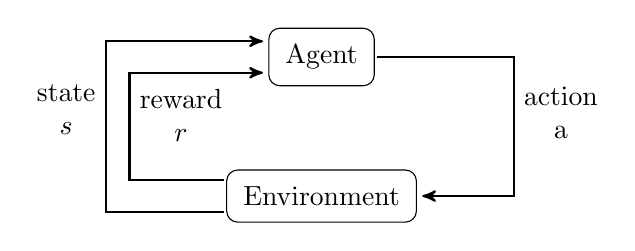
\begin{tikzpicture}
		\node [block] (agent) {Agent};
		\node [block, below=of agent] (env) {Environment};
		\draw [flow] ([yshift=2mm]env.west) -- ++(-1.2,0) |-
			([yshift=-2mm]agent.west) node [pos=0.3,right] {reward\\$r$};
		\draw [flow] ([yshift=-2mm]env.west) -- ++(-1.5,0) |-
			([yshift=2mm]agent.west) node [pos=0.3,left] {state\\$s$};
		\draw [flow] (agent.east) -| node [pos=0.7,right] {action\\a}
		($(env.east)+(1.2,0)$) -- (env.east);
	\end{tikzpicture}
	\caption{How agent and environment interact in RL.}
	\label{fig:rl}
\end{figure}


\subsection{Markov Decision Processes}

% MDP
Most RL algorithms assume that the environment dynamics can be modelled with a
\emph{Markov Decision Process} (MDP)\nomenclature{MDP}{Markov Decision
Process}. They do so, because under the independence assumptions taken by MDP,
it's possible to efficiently find the optimal agent's policy.

\begin{definition}
	A Markov Decision Process is a tuple $\langle \stateS, A, T, R, \discount
	\rangle$, where: $\stateS$ is the set of states of the environment; $A$ is
	the action space; $T: \stateS \times A \times \stateS \to \R$ is the
	transition function, which, for ${T(s_{t}, a_{t}, s_{t+1})}$, returns the
	probability $p(s_{t+1} \given s_{t}, a_{t})$ of the transition ${s_{t}
	\xrightarrow{a_{t}} s_{t+1}}$; $R: \stateS \times A \times \stateS \to \R$
	is the reward function; and $\discount \in [0, 1]$ is called ``discount
	factor''\footnote{In this chapter, variables with an integer subscript or
	index refer to the value at the discrete time indicated.}.
\end{definition}

% Markov assumptions
In a RL problem, the functions $T$ and $R$ are unknown. The agent can only
learn them by taking each action and observing the outcomes. Even if they are
unknown, by assuming that they can be modelled with functions ${\stateS \times
A \times \stateS \to \R}$, we introduce some Markov assumptions. In
particular, we assume that the next state of the environment is conditionally
independent on the whole history, given the previous state and action:
$s_{t+1} \perp s_{0}, \dots, s_{t-1} \given s_{t}, a_{t}$. Similarly, the
reward only depends on the last transition of the environment.  Although it's
not required by the model, it is common that rewards are computed just from
desirable configurations of the environment~$s_{t}$, not from specific
transitions $(s_{t-1}, a_{t-1}, s_{t})$. All these assumptions are summarized
in the Directed Graphical Model (DGM)\nomenclature{DGM}{Directed Graphical
Model} of Figure~\ref{fig:mdp}. In a DGM, edges indicate direct conditional
probabilities, while missing arcs indicate conditionally independent
variables.  In Figure~\ref{fig:mdp}, the lack of any arrow between $s_{t-1}$
and $s_{t+1}$ means that future states, hence the rewards, do not depend on
the past history, given the current state~$s_t$.  This is the essence of a
Markov assumption.

\begin{figure}
	\centering
	\begin{tikzpicture}
		\matrix [
			column sep={1cm,between origins}, row sep={1cm,between origins},
		] {
			\&
			\node (am1) [observed node, label=above:$a_{t-1}$] {};
			\& \&
			\node (a) [observed node, label=above:$a_{t}$] {}; \& \\
			\node (stm1) [observed node, label=above:$s_{t-1}$] {};
			\& \&
			\node (st) [observed node, label=above:$s_{t}$] {}; \& \&
			\node (st1) [observed node, label=above:$s_{t+1}$] {}; \\
			\& \&
			\node (r) [observed node, label=below:$r_{t}$] {}; \& \&
			\node (r1) [observed node, label=below:$r_{t+1}$] {}; \\
		};
		\draw (st1) edge [<-] (st) edge [<-] (a);
		\draw [->, dotted] (st) -- (a);
		\draw [->] (st) -- (r);
		\draw [->] (st1) -- (r1);
		\draw (st) edge [<-] (stm1) edge [<-] (am1);
		\draw [->, dotted] (stm1) -- (am1);

		\draw [dashed, gray] (st1) -- +(0.8,0);
		\draw [dashed, gray] (stm1) -- +(-0.8,0);
	\end{tikzpicture}
	\caption{The directed graphical model of an MDP.}
	\label{fig:mdp}
\end{figure}

\begin{example}
	\label{ex:board-games}
	Tic-Tac-Toe, Chess and many other board games can be modelled with an MDP.
	Even games with dice, such as Backgammon. To do so, we define as state
	space~$\stateS$ the set of configurations of the board, and a reward
	function $R(s)$ that returns $1$, if the configuration $s$ is a win, $-1$
	for a loss, and 0 otherwise. Even though most games are deterministic, the
	presence of an opponent makes the transition function~$T$ of the MDP
	nondeterministic.  What these games have in common, is that the player gets
	to see the complete state of the game, which is the current configuration of
	the board. Future states of the game and rewards only depend on the current
	situation, not on the whole play. In Chess, for example, we can determine
	whether a configuration is a win or loss just by looking for a checkmate;
	there is no need to ask the players how the game has been carried out.

	Proving that Markovian $T$ and $R$ exist is easy for board games, because
	the rules of the game define them. As we will see in
	Section~\ref{sec:non-markov}, when $T$ is unknown, as always happens in the
	real-world, it's much more difficult to prove that we're in fact facing an
	MDP.
\end{example}


\subsection{Optimal policies}

The \emph{policy} is the criterion the agent uses to select the actions to
perform. If the environment dynamics can be modelled with an MDP, the
optimal action at time~$t$ only depends on~$s_{t}$. So, there must exist
an optimal policy as $\optimal\policy: \stateS \to A$. However, due to common
estimation errors, it is always better to prefer nondeterministic policies,
which return a probability distribution over the actions. The action at time
$t$ will be sampled according to $a_t \sim \policy(s_t)$. This dependency is
represented by the dotted arrows of Figure~\ref{fig:mdp}. A policy that is a
function only of the state is called ``stationary''.

We will now introduce few basic quantities of RL that serve to define what it
means for an action or a policy to be optimal. The \emph{discounted
return}~$G$ is the combination of all rewards collected:
\begin{equation}
	G \coloneqq r_{0} + \discount\, r_1 + \discount^2 r_2 + \dots =
	\sum_{t=0}^{T} \discount^{t} r_{t}
	\label{eq:return}
\end{equation}
The discount factor, $0 \le \discount \le 1$, decides the relative importance
of immediate and future rewards. Usually, this factor is strictly less than 1
because this stimulates the agent to achieve rewards as soon as possible.
It also produces a finite discounted reward, even for an infinite run, where
$T \to \infty$.  Since the environments we will experiment with are video
games, each play is an episode and the total number of steps in each episode
is finite.

It is now clear, that the optimal policy should always maximize the expected
discounted return. The \emph{value function} of a policy $\policy$ computes
this quantity from each state $s$:
\begin{equation}
	v_{\policy}(s) \coloneqq \E_{\policy}[G \given s_0 = s]
	\label{eq:mdp-value}
\end{equation}
which is the expected value of $G$, when the agent starts from state $s$
and it follows the policy~$\policy$. The notation $\E_{\policy}$ indicates
that the estimation assumes that the actions are sampled according
to~$\policy$. Finally, we can define the \emph{optimal policy}
$\optimal\policy$ as the one maximizing the value function at all states:
\begin{equation}
	\optimal\policy: \quad v_{\optimal\policy}(s) \ge v_{\policy}(s) \qquad
	\forall s \in \stateS, \quad \text{for all $\policy$}
\end{equation}
The typical Reinforcement Learning problem is to find the optimal policy for
an MDP with unknown $T$ and~$R$.

The \emph{action-value function} of a policy $\policy$ is a similar measure to
the value function:
\begin{equation}
	q_{\policy}(s, a) \coloneqq \E_{\policy}[G \given s_0 = s, a_0 = a]
\end{equation}
which also forces the first action to be~$a$. Since the agent can only observe
outcomes of single actions, this is usually a much more convenient form for
updating the estimate of the expected discounted return. Most important, the
optimal policy can be simply expressed as:
\begin{equation}
	\optimal\policy(s) = \argmax_{a \in A} q_{\optimal\policy}(s, a)
	\label{eq:opt-policy-q}
\end{equation}
So, instead of learning the optimal policy directly, we can learn the optimal
state-value function,~$q_{\optimal\policy}$ (also denoted with $\optimal{q}$).
Fortunately, we don't need $\optimal\policy$ to valuate $\optimal{q}$ because,
assuming optimality, we know it satisfies the Bellman optimality equation:
\begin{align}
	\optimal{q}(s, a) &= \E\, \bigl[ r_{t+1} + \discount \max_{a'}
	\optimal{q}(s_{t+1}, a') \given s_t = s, a_t = a \bigr] \\
	&= \sum_{s', r'} p(s', r' \given s, a) \,
	\bigl( r' + \discount \max_{a'} \optimal{q}(s', a') \bigr)
	\label{eq:q-bellman}
\end{align}
for any~$t$.

Many learning algorithms exist for estimating $\optimal{q}$. Briefly, on-policy
algorithms, estimate $q_\policy$ of the policy $\policy$ that is being used
and improved, $\policy \to \optimal\policy$; off-policy algorithms, instead,
act according to any exploration policy $\policy_e$ and directly estimate
$\optimal{q}$.  Two famous algorithms in these classes are SARSA and
Q-learning, respectively.  The one used in this thesis is derived from the
latter.


\subsection{Exploration policies}

\label{sec:exploration-policies}

If $\optimal{q}$ were know, equation~\eqref{eq:opt-policy-q} would be enough
to always select the optimal action. Generalizing for any $q$, we call that
the \emph{greedy policy}, because it always selects the best action according
to $q$:
\begin{equation}
	\policy_q(s) \coloneqq \argmax_{a \in A} q(s, a)
	\label{eq:pol-greedy}
\end{equation}
Unfortunately, while learning, we only have a rough estimate of the optimal
function, ${\est{q} \approx \optimal{q}}$. Being greedy with respect to
sub-optimal policies is dangerous, because the agent may deterministically
select actions that repeatedly lead to dead-ends.  To mitigate this issue, we
can choose some actions at random. The \emph{\eps-greedy policy} is defined
as:
\begin{equation}
	\policy_{q,\epsilon}(s) \coloneqq
	\begin{cases}
		\text{random action $a \in A$}
		&\text{with probability $\epsilon$} \\
		\argmax_{a \in A} q(s, a)
		&\text{otherwise}
	\end{cases}
	\label{eq:pol-eps}
\end{equation}
More precisely, random actions are sampled from a uniform distribution over
the set of actions $A$. By making random moves, the agent might escape from
suboptimal environment configurations. If $\epsilon = 1$,
definition~\eqref{eq:pol-eps} reduces to the random policy:
\begin{equation}
	\policy_r(s) \coloneqq \text{random action $a \in A$}
	\label{eq:pol-random}
\end{equation}

When training begins, the agent has no clue about the optimal q-function. It
can just try out all actions by executing the random policy. In this phase,
the agent receives low rewards but observes a lot of different outcomes for
its actions. This is the purpose of exploration. After a while, the agent can
begin to trust in its predictions. So, it may gradually choose the most
promising actions in order to achieve higher rewards. This is the exploitation
phase.  The exploitation--exploration trade-off is a fundamental problem in
AI.  Unfortunately, there's no general solution in RL, because the agent has
no way to tell when the policy is ``good enough''. Usually, we need to try
some compromises between the two.

To address this issue, during training, the agent can act according to a
policy that is initially stochastic but gradually approaches the greedy
policy, over time. There are many ways to do this. One of the most simple
options is to select the \eps{}-greedy policy of equation~\eqref{eq:pol-eps}
with \eps{} that varies over time according to some schedule.
Figure~\ref{fig:policy-schedules} shows two common possibilities.
\begin{figure}
	\centering
	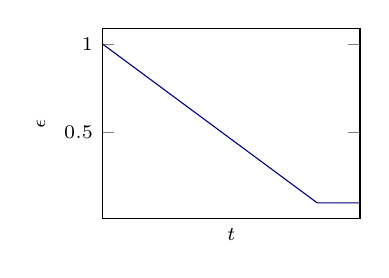
\begin{tikzpicture}
		\begin{axis}[
				xmin=0, xmax=120, width=0.4\textwidth, height=4cm,
				xlabel=$t$, ylabel=\eps{}, xtick=\empty]
			\addplot [blue!50!black] coordinates {
				(0, 1)
				(100, 0.1)
				(120, 0.1)
			};
		\end{axis}
	\end{tikzpicture}
	\qquad
	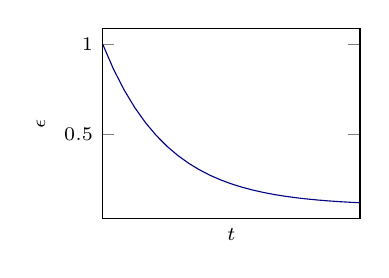
\begin{tikzpicture}
		\begin{axis}[
				xmin=0, xmax=120, width=0.4\textwidth, height=4cm,
				xlabel=$t$, ylabel=\eps{}, xtick=\empty]
			\addplot [blue!50!black, domain=0:120] {
				0.9*exp(-x/30)+0.1
			};
		\end{axis}
	\end{tikzpicture}
	\caption{Probability of a random action over time: \eps{} with linear decay
	(left), \eps{} with exponential decay (right).}
	\label{fig:policy-schedules}
\end{figure}
On the left-hand figure, the probability of a random action is linearly
decreased over time, while on the right, it follows an exponential decay. In
both cases \eps{} never becomes zero, because that would effectively terminate
the learning process. The rate of this decrease is a hyperparameter that
can be tuned.

The most common policies are those just described. They can be directly
used in a RL algorithm or combined to create more complex policies. With
``exploration policy'' we refer to any policy that has a strong component of
nondeterminism and it's suitable to drive the agent's behaviour during
training.


\subsubsection*{Custom exploration policies}

We'll now define few other policies which we proposed and used in this
thesis. Of course, there is no better policy in general. The policies defined
here might be suitable for the environments we face, but may be inappropriate
in many others. They just happen to be useful for one class of environments.

The first one is an $\epsilon$-greedy policy with action repetition. It
chooses between random and deterministic actions just like the
$\epsilon$-greedy. However, consecutive random moves always execute the same
action. This sequence of repetitions can be interrupted by a deterministic
move or by the threshold of maximum repetitions. This policy may be useful in
environments where the effect of a single action is very small. This is the
case, for example, for the exploration of mazes and corridors. The random
policy wouldn't allow the player to cover large distances, because of the
uniform sampling between left and right.

The second policy is an $\epsilon$-greedy with random~$\epsilon$. As we will
see in Section~\ref{sec:training-incremental}, when we need to observe the
environment dynamics, we need to see the observations received in response to
many different stimuli. However, when we apply $\epsilon$-greedy to a capable
agent, we see the following pattern: $\epsilon$ determines the agent's
ability. To a fixed $\epsilon$ corresponds some average ability, and the
cumulative rewards achieved tend to be very similar. Following this intuition,
we define a policy that samples a random $\epsilon$ for each episode.
So, at different episodes, the agent can explore both the early stages and
more distant environment states.

The last policy we define addresses the same problem as the previous one,
producing very diverse trajectories, but in environments with sparse rewards.
When the reward is sparse, we can read it as successful completion of some
sub-task. In this policy, for each episode, we sample a random natural number,
that we call ``checkpoint''. When the number of rewards collected is lower
than the checkpoint, the agent behaves mostly in a deterministic way, because
the purpose is just to proceed. When the number of rewards reaches the
checkpoint number, we act according to a random policy. The idea is to explore
the environment state space at different depths.


\section{Deep Reinforcement Learning}

\label{sec:deep-rl}

Classic RL algorithms, such as SARSA and Q-learning, are tabular methods.
In fact, they store and update the estimate for each pair $(s, a)$
independently. Unfortunately, this requires discrete and small states and
actions spaces. To overcome this very limiting assumption, we need
parametrized value functions and policies.  \emph{Deep Reinforcement Learning}
(Deep RL) is a recent field of RL in which Neural Networks
(NN)\nomenclature{NN}{Neural Network} are used as powerful function
approximators for policies or value functions.

The main advantage of NNs, and parametric models in general, is that they can
be trained in high-dimensional and continuous input spaces. In fact, a good
fit does not require a complete exploration of the input space, which may be
unfeasible or impossible. Instead, they are trained with some form of
Stochastic Gradient Descent on the set of parameters from input-output
samples. Then, the model can be able to generalize to inputs that have been
never observed, in a meaningful way.

Unfortunately, due to approximation and parametrization, Deep RL algorithms
allow very little guarantees about convergence and optimality. Even if the
input space would be explored completely, updates for recent samples would
also affect the regions previously visited. In fact, any effective Deep RL
algorithm introduces some techniques in order to generate a stable training.


\subsection{Environment: Atari 2600 games}

\label{sec:atari-envs}

The Atari 2600 is a video game platform that was developed in 1977. There are
hundreds of classic games available to play: Space Invaders, Ms. Pacman,
Breakout and many others. The screen is 160 pixels wide and 210 pixels high,
with RGB colors of 8-bits depth. The joystick has 9 positions (3 for each
axis) and one button, for a total of 18 possible actions. For this reason,
we'll only focus on RL methods for discrete action spaces.

The Arcade Learning Environment~\cite{bib:atari-games} is a simple interface
to the Atari 2600 emulator. It allows agents to play and be trained on these
games. At each step, the agent chooses one of the 18 actions available and
receives in return a frame of the game and a reward. The reward is the
increment in the player's score for the original game. This is really the same
interface that a human player would use. Figure~\ref{fig:atari-frames} shows
the frames from few games in this collection. 

\begin{figure}
	\centering
	\includegraphics[width=0.25\textwidth]{./imgs/si0.png}
	\quad
	\includegraphics[width=0.25\textwidth]{./imgs/br0.png}
	\quad
	\includegraphics[width=0.25\textwidth]{./imgs/mz0.png}
	\caption{Initial frames of some Atari 2600 games (left to right): Space
		Invaders, Breakout, Montezuma's Revenge.}
	\label{fig:atari-frames}
\end{figure}

Although these games come from an early stage of video games development, they
represent the appropriate challenge for current (Deep) Reinforcement Learning
agents. In fact, many papers tested their RL algorithms on these
games~\cite{bib:atari-deeprl}%
\cite{bib:atari-deepq-nature}\cite{bib:double-q}\cite{bib:rainbow}.
In this thesis, we also tested with some of these environments. We will also
show how improve on the hardest game in this collection for a RL agent:
Montezuma's Revenge.


\subsection{Deep Q-Network}

\label{sec:deep-q-agents}

The \emph{Deep Q-Network} (DQN)\nomenclature{DQN}{Deep Q-Network
algorithm}~\cite{bib:atari-deeprl} was the first algorithm to successfully
combine deep learning models and Reinforcement Learning. Although many basic
ideas presented here have been already introduced by the Neural Fitted
Q~iteration algorithm~\cite{bib:nfq}, DQN addressed some causes of training
instability. They also demonstrated that exactly the same agent can be trained
in many Atari games and achieve human-level performances in many of
those~\cite{bib:atari-deepq-nature}. These promising results sparked a lively
interest in Deep RL, recently.

In DQN, the state-action value is approximated by a deep neural network ${Q(s,
a; \param)}$, on the parmeters $\param$, that we call Q-Network. The purpose
of learning, is to train this network to approximate the optimal q-function: 
$\est{\param}: Q(s, a; \est{\param}) \approx \optimal{q}(s, a)$. Then, the
estimated optimal policy will be:
\begin{equation}
	\est{\policy}(s) = \argmax_{a \in A} Q(s, a; \est{\param})
\end{equation}

A trained network, for each input $(s, a)$, should return the expected value
of some target~$y_{s,a}$. To do so, we select the parameters that minimize the
squared difference between the estimates and the targets:
\begin{equation}
	\text{loss}(\param) \coloneqq \bigl(Q(s, a; \param) - y_{s,a} \bigr)^2
	\label{eq:qnet-generic-loss}
\end{equation}
Since this is a Q-Network, the targets are the optimal state-action
values~$\optimal{q}(s, a)$ that the net should estimate.  The
loss~\eqref{eq:qnet-generic-loss} contains some random variables. So, we
minimize it through any stochastic optimization algorithm. In Stochastic
Gradient Descent (SGD)\nomenclature{SGD}{Stochastic Gradient Descent
algorithm}, at each step $t$, we observe an input ${(s_t, a_t)}$ and the
associated target $y_t$. Then, we take a small step toward the negative
gradient of the loss:
\begin{equation}
	\param_{t+1} = \param_t - \alpha\, \nabla_{\param}\,
	\Bigl( \bigl(Q(s_t, a_t; \param) - y_t \bigr)^2 \Bigr) \Big|_{\param =
	\param_t}
	\label{eq:sgd-update}
\end{equation}
in which $0 < \alpha < 1$ is a small learning rate. This equation is not
the only update rule possible. There are more advanced optimization
algorithms, such as: Momentum, RMSprop and Adam. In this thesis, we've
mostly experimented with Adam.

What has just been described is the usual way of fitting a neural network
to a dataset of samples. In RL, however, the targets $\optimal{q}(s_t, a_t)$
are unknown, because they depend recursively from the same optimal q-function
that we're trying to learn (see equation~\eqref{eq:q-bellman}). In classic RL,
this is not a problem: the 1-step approximation of the q-values (derived from
equation~\eqref{eq:q-bellman}),
\begin{equation}
	y_t \coloneqq r_{t+1} + \discount \max_{a \in A} \est{q}(s_{t+1}, a)
	\label{eq:1step-targets}
\end{equation}
or the n-step approximation, are a valid targets for the function~$\est{q}$.
By updating toward these values on the whole input space, convergence is
guaranteed. In other words, targets can be estimates themselves.

With neural networks, instead, any update to the parameters also affects the
target, because the weights have a global influence on the function. It's not
possible apply a correction for just one tiny region of the input space (nor
it's desirable, after all).  It has been shown~\cite{bib:nfq}, that due to
this effect, propagating errors slow down convergence or even render the
training unstable.  To address this issue one must ensure that the targets do
not move much.

The DQN~\cite{bib:atari-deeprl} algorithm addresses this issue in two ways.
First, the targets in equation~\eqref{eq:1step-targets} are not generated by
the network that is being trained, $Q(s, a; \param)$, but they are computed
from a second net, $Q(s, a; \param')$. Every $C$ iterations, the target net
is updated to match the trained net, with the assignment: $\param' \gets
\param$. This keeps the targets constant for $C$ steps and helps to stabilize
the training.

Second, the network is not trained from the last sample, but from transitions
of the recent experience. At each step, the agent acts according to some
exploration policy, $a_t \sim \policy_e$. Each transition, of the form
$\langle s_t, a_t, r_{t+1}, s_{t+1} \rangle$, is recorded in a buffer of size
$n_r$, called ``experience replay''. Then, at each training step, we sample a
number of $n_b$ transitions, thus creating a batch, and we perform an update
$\param_{i+1} = \param_i - \alpha\, g_i$ on the cumulative gradient $g_i$ of
the whole batch.

DQN also includes a number of heuristics that greatly help the training
but are specific to the Atari~2600 environments:
\begin{itemize}
	\item Rewards can be really high, so they are limited in the range $[-1,
		+1]$; this is called \emph{reward clipping}. It helps to keep the same
		learning rate for diverse games.
	\item The agent has a single life available. When a life is lost, the
		episode ends. This prevents the agent to rely on restarts.
	\item The frames are slightly down-scaled to further reduce the resolution,
		they are transformed to gray-scale and mapped to the range $[-1, +1]$.
		These are common preprocessing steps for NNs.
	\item Every observation is composed by the last 4 frames stacked together.
		This allows the agent to observe how the objects in the scene move.
		See Section~\ref{sec:non-markov} and Example~\vref{ex:motion}.
\end{itemize}

The algorithm used in this thesis is called \emph{Double
DQN}~\cite{bib:double-q}. It is a slight variant of DQN, so all details
mentioned so far also apply. The motivation of this algorithm is a known issue
of Q-learning: it is likely to make overoptimistic value estimates.
To show this, let's rewrite the targets of~\eqref{eq:1step-targets} as:
\begin{equation}
	y_t \coloneqq r_{t+1} + \discount \, Q(s_{t+1}, \argmax_{a \in A} Q(s_{t+1},
	a; \param_t); \param_t)
\end{equation}
where the estimates $\est{q}$ are computed with the Q-Network. This form makes
more evident that the same model is used both to select the next greedy action
and to estimate the q-value of state~$s_t$. As result, any action with an
overestimated q-value will be selected and its value propagated. To remove
this bias, Double DQN decouple the two operations by using different sets of
parameters, $\param\group{1}$ and $\param\group{2}$. The targets $y_t$ are
computed as:
\begin{equation}
	y_t \coloneqq r_{t+1} + \discount \, Q(s_{t+1}, \argmax_{a \in A} Q(s_{t+1},
	a; \param_t\group{1}); \param_t\group{2})
	\label{eq:double-q-targets}
\end{equation}
Then, just the parameters $\param\group{1}$ are updated toward this targets;
this is called the online network. With random chance, the roles of the two
parameters are continuously swapped at each step.

To compute the target, we need to compute the q-values for all actions in
state $s_{t+1}$. To speed up this computation, the network is defined as a
function that takes in input a state and computes a vector of state-action
values, one for each action. So, just one forward pass is required to select
the next action. Common Q-Networks for images are composed of a number of
convolutional layers and some fully-connected layers. The specific structure
may change, and the network used will be defined in the implementation section.


\section{Non-Markovian goals}

\label{sec:non-markov}

The goal of a RL agent is to maximize the rewards received.  A goal, or a
task, is said \emph{non-Markovian} if the rewards do not satisfy the Markov
assumption on rewards, i.e:
\begin{equation}
	r_{t+1} \not\perp s_i, a_i, r_i \given s_t, a_t
	\qquad \text{for some $t, i$, with $0 \le i < t$}
	\label{eq:markov-rewards}
\end{equation}
Of course, this can happen only if the environment cannot be modelled with an
MDP. Excellent algorithms exists for MDPs; instead, non-Markovian goals are
much more difficult to learn.  There are two main causes for non-Markovian
rewards: partial observations and temporally-extended tasks. We'll thoroughly
analyze both scenarios.


\subsection{Partial observations}

\label{sec:partial-obs}

Up to this point, we didn't need to distinguish between observations and
states. In fact, we assumed that the agent can directly observe the
environment states and act accordingly (we defined the policy as a function of
the state). Unfortunately, this is often not the case: we only get to see
something that depends on the current state, but it's not. These systems can
be modelled with a \emph{Partially Observable Markov Decision Process}
(POMDP)\nomenclature{POMDP}{Partially Observable Markov Decision Process}.
POMDPs are a generalization of MDPs for partial observations. From now on, we
will denote with $\stateS$ the environment state space and with $\obsS$ the
observation space. Formally, a discrete-time POMDP is a 7-tuple ${\langle
\stateS, A, T, R, \obsS, O, \discount \rangle}$, where $\stateS, A, T, R$ are
defined as in MDPs, $\obsS$ is the observation space, and $O$ is the
observation function ${O: S \to \obsS}$.

The graphical model of a POMDP is shown in Figure~\ref{fig:pomdp}.
\begin{figure}

	\centering
	\begin{tikzpicture}
		\matrix [
			column sep={1.5cm,between origins}, row sep={1cm,between origins},
		] {
			\node (om1) [observed node, label=above:$o_{t-1}$] {}; \&
			\node (am1) [observed node, label=above:$a_{t-1}$] {}; \&
			\node (o) [observed node, label=above:$o_{t}$] {}; \&
			\node (a) [observed node, label=above:$a_{t}$] {}; \\
			\node (stm1) [node, label=below left:$s_{t-1}$] {};
			\& \&
			\node (st) [node, label=below left:$s_{t}$] {}; \& \&
			\node (st1) [node, label=below left:$s_{t+1}$] {}; \\
			\& \&
			\node (r) [observed node, label=below:$r_{t}$] {}; \& \&
			\node (r1) [observed node, label=below:$r_{t+1}$] {}; \\
		};
		\draw [->] (stm1) -- (om1);
		\draw [->] (st) -- (o);
		%
		\draw [->] (st) -- (r);
		\draw [->] (st1) -- (r1);
		%
		\draw [->, dotted] (om1) -- node [midway] {?} (am1);
		\draw [->, dotted] (o) -- node [midway] {?} (a);
		%
		\draw (st) edge [<-] (stm1) edge [<-] (am1);
		\draw (st1) edge [<-] (st) edge [<-] (a);

		\draw [dashed, gray] (st1) -- +(0.8,0);
		\draw [dashed, gray] (stm1) -- +(-0.8,0);
	\end{tikzpicture}
	\caption{The Directed Graphical Model of a POMDP. White nodes are
	unobservable. For simplicity, the rewards in this graph depend just on the
	current state $s_t$, not on transitions ${(s_t, a_t, s_{t+1})}$.}
	\label{fig:pomdp}
\end{figure}
The sequence of states ${\langle s_0, s_1, \dots \rangle}$, which is the
environment dynamics, still satisfies the Markov assumption (it forms a Markov
chain). In a POMDP, this dynamics exists but is unobservable. What we can
see, instead, is a sequence of observations ${ \langle o_0, o_1, \dots
\rangle}$. Each of them is generated from the corresponding state, through the
(possibly nondeterministic) observation function. Actions and policies can
only act in response to observations, not states.

The dotted arrows in Figure~\ref{fig:pomdp} have a question mark on them,
because that dependency is our choice. As designers, we're free to select
the informations that the agent should take into account when selecting an
action. Is the last observation enough to decide? Or, more precisely, among
all possible policies, do non-Markovian goals always admit an optimal policy
of the form $\optimal\policy: \obsS \to A$? Unfortunately, the answer is no.
As we will see, other informations are needed.

If the transition and observation functions are known, a common solution is to
estimate the states and decide the action from this belief. With deterministic
functions, the agent can iteratively restrict the set of possible states by
eliminating those inconsistent with the observations received. More commonly,
these functions are nondeterministic. In this case, probabilistic methods
can be effective estimation algorithms. The iterative probabilistic filter
applied to the sequence of observations would produce the belief distribution
of the current state.  We can represent the general procedure, at any
instant~$t$, with the following computation:
\begin{center}
	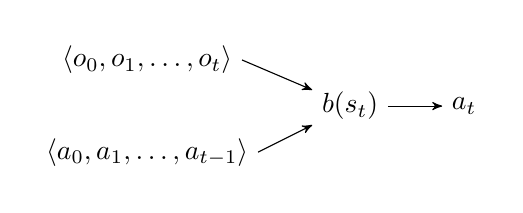
\begin{tikzpicture}
		\matrix [column sep=2em] {
			\node (o) {$\langle o_0, o_1, \dots, o_t \rangle$}; \\
			\&
			\node (s) {$b(s_t)$}; \& \node (an) {$a_t$}; \\
			\node (a) {$\langle a_0, a_1, \dots, a_{t-1} \rangle$}; \\
		};
		\draw [->] (o.east) -- (s);
		\draw [->] (a.east) -- (s);
		\draw [->] (s) -- (an);
	\end{tikzpicture}
\end{center}
where $b(s)$ denotes the belief of $s$, being either a set of states or a
probability distribution. Since these beliefs depend on the whole sequence of
observations, also the next action is implicitly based on the whole history.

Standard RL algorithms cannot be applied to POMDPs, because the state space is
not observable. Also, since we commonly assume the transition and observation
functions to be unknown, no estimation could be carried out anyway.  There is
a clear difference between MDPs and POMDPs. Still, RL algorithms are
frequently applied to POMDPs. Not surprisingly, they perform very poorly on
these environments. See, for example, the games with worst performances
in~\cite{bib:atari-deepq-nature}. This is a subtle mistake, because
determining whether we're observing the state space is the same as answering
the following question: does the observation space capture the whole dynamics
of the system? Or, more precisely, does an equivalent MDP $\langle \obsS, A,
T_\obsS, R_\obsS, \discount' \rangle$, that produces the same rewards, exist?
If both $T_\obsS: \obsS \times A \times \obsS \to \R$ and $R_\obsS: \obsS
\times A \times \obsS \to \R$ exist and produce the same rewards, the
environment can be successfully modelled and solved with an MDP.
Figure~\ref{fig:pomdp-as-mpd} represents this situation.

\begin{figure}
	\centering
	\begin{tikzpicture}[
			hidden arc/.style={->, densely dotted},
			box/.style={rounded corners=5pt, inner sep=1.8ex, draw=#1!50,
				fill=#1!20},
		]
		\matrix [
			column sep={1.6cm,between origins}, row sep={1.3cm,between origins},
		] {
			\node (stm1) [node, label=above:$s_{t-1}$] {}; \& \&
			\node (st) [node, label=above:$s_{t}$] {}; \& \&
			\node (st1) [node, label=above:$s_{t+1}$] {}; \\
			\&
			\node (am1) [observed node, label=above:$a_{t-1}$] {}; \&
			\node (r) [observed node, label=left:$r_{t}$] {}; \&
			\node (a) [observed node, label=above:$a_{t}$] {}; \&
			\node (r1) [observed node, label=left:$r_{t+1}$] {}; \\
			\node (om1) [observed node, label=below:$o_{t-1}$] {}; \& \&
			\node (o) [observed node, label=below:$o_{t}$] {}; \& \&
			\node (o1) [observed node, label=below:$o_{t+1}$] {}; \\
		};
		\draw [hidden arc, bend left] (stm1) to (om1);
		\draw [hidden arc, bend left] (st) to (o);
		\draw [hidden arc, bend left] (st1) to (o1);
		%
		\draw [hidden arc] (st) -- (r);
		\draw [hidden arc] (st1) -- (r1);
		%
		\draw [hidden arc] (stm1) -- (st);
		\draw [hidden arc] (st) -- (st1);
		\draw [hidden arc] (am1) -- (st);
		\draw [hidden arc] (a) -- (st1);
		%
		\draw [dashed, gray] (st1) -- +(0.8,0);
		\draw [dashed, gray] (stm1) -- +(-0.8,0);
		%
		\draw [->] (o) -- (r);
		\draw [->] (o1) -- (r1);
		%
		\draw [->] (om1) -- (o);
		\draw [->] (o) -- (o1);
		\draw [->] (am1) -- (o);
		\draw [->] (a) -- (o1);
		%
		\draw [dashed, gray] (st1) -- +(0.8,0);
		\draw [dashed, gray] (stm1) -- +(-0.8,0);
		\draw [dashed, gray] (o1) -- +(0.8,0);
		\draw [dashed, gray] (om1) -- +(-0.8,0);
		% boxes
		\begin{pgfonlayer}{below}
			\path coordinate (st-up) at ($(st)+(0,1em)$);
			\node [fit={(stm1) (st1) (st-up)}, box=gray,
				pin=right:{\footnotesize hidden dynamics}
			] {};
			\node [fit={(om1) (o1) ($(a.north)+(0,1ex)$) ($(o.south)+(0,-1ex)$)},
				box=orange, pin=right:{\footnotesize MDP assumption}] {};
		\end{pgfonlayer}
	\end{tikzpicture}
	\caption{The dotted arrows \protect\tikz [baseline=-0.5ex] \protect\draw
	[densely dotted, ->] (0,0) to +(1.5em,0); represent the dependencies in a
	POMDP model. Solid arrows \protect\tikz [baseline=-0.5ex] \protect\draw
	[->] (0,0) to +(1.5em,0); show the MDP model over the same quantities.}
	\label{fig:pomdp-as-mpd}
\end{figure}

\begin{example}
	As we've seen from Example~\vref{ex:board-games}, the game of Chess can
	be modelled with an MDP if we consider as states the vectors of positions of
	all pieces on the board. Let's suppose, instead, the observations available
	are images of the board after each move (if the pieces can be distinguished,
	these could even come from a real play). Each image completely captures the
	state of the game because, for each move of the agent and the opponent,
	we're able to accurately predict the image that will follow. This is a
	transition $T_\obsS$ over images. Similarly, a reward function $R_\obsS$ can
	simply return $+1$ or $-1$ for images with checkmates and 0 otherwise. These
	functions can be unknown and don't need to be defined.

	Suppose, instead, that the agent can only observe the left-hand side of the
	board (columns a-d, for example). In this case, each image provides an
	incomplete view over the state of the game. In fact, in order to determine
	the best action we must consider whether there are some attacking pieces on
	the hidden region. In this case, classic RL algorithms would perform poorly,
	because without any memory about the position of the hidden pieces, 
	it's not possible to predict the next image and reward from the current
	observation.
	\label{ex:chess-partial-obs}
\end{example}

\begin{example}
	Let's consider a classic control problem: the swing-up of an inverted
	pendulum. A pendulum can freely rotate by 360° around a hinge. The agent, at
	each discrete time step, can apply torques to this active joint.  The goal
	is to stabilize the pendulum in the upward position, which is the
	configuration of unstable equilibrium. In order to solve this problem with
	Reinforcement Learning, we need to define the spaces $S$ and $A$ of the MDP.
	In this domain, actions are continuous torques, which may be represented in
	a normalized range: $A \coloneqq [-1, +1] \subseteq \R$. The angle of the
	pendulum $\theta$ with respect to some fixed reference completely determines
	the position of the masses. Is the reward Markovian with respect to $S
	\coloneqq \{\theta \in [-\pi, +\pi]\}$? No, because the agent is rewarded
	when the pendulum \emph{stops} in the upward position. So, the appropriate
	state space consists of both $\theta$ and $\dot\theta$ (or, rather its
	discrete-time approximation).

	Including the momentum in the state space is very common for mechanical
	systems. However, this can be also necessary for games. In fact, just
	looking at a single frame, the agent has no clue about how all the elements
	in the picture are moving.  For example, in a video game where the agent has
	to hit a moving ball, the optimal policy certainly needs to observe also its
	direction.
	\label{ex:motion}
\end{example}


\subsection{Temporally-extended goals}

\label{sec:tempoal-goals}

The previous section has shown how partial observations may falsify the Markov
assumption on rewards. A second possibility is to have a complete observation
of the state ($\obsS = \stateS$) but a task that is intrinsically
non-Markovian. In this case, each reward is computed from the whole history
of events
\begin{equation}
	r_t = R(\langle s_0, s_1, \dots, s_t \rangle) \qquad \forall t \in \Z
	\label{eq:nm-rewards}
\end{equation}
with $R: \stateS^* \to \R$. The sequence of states $\trace
\coloneqq \langle s_0, s_1, \dots, s_t \rangle$ will be also called
execution \emph{trace}. In general, with the term ``trace'' we indicate any
sequence that is produced during a run. We adopt a similar notation to those
we've seen for interpretations of temporal logics.

Goals defined by rewards of equation~\eqref{eq:nm-rewards} are said
``temporally-extended'' because they take into account multiple timesteps. Why
should we define a reward function that is explicitly non-Markovian? One
possibility is that we might want our agent to drive the environment through a
\emph{sequence} of states, instead of just reaching a single configuration.
However, as we will see, we don't need to restrict to sequences, because we
may define very complex reward functions.

\begin{example}
	Let's suppose the agent can control a light bulb through a switch, and we
	want the light to be set on, then off again. The agent will be rewarded if,
	at the end of the episode, the light has been set on only once.  The
	environment is extremely simple: its state may be completely described by a
	Boolean variable, ``lightOn'', which reflects the status of the light.
	Still, in order to valuate whether the task has been accomplished, it's not
	sufficient to check whether the light is off at the end of the episode; we
	also need to ensure that, \emph{during the whole episode}, it has been
	switched on only once.
	\label{ex:light}
\end{example}

We now define a model that, by generalizing MDPs, can describe this large
class of problems.
\begin{definition}
	A \emph{Non-Markovian Reward Decision Process}
	(NMRDP)\nomenclature{NMRDP}{Non-Markovian Reward Decision
	Process}~\cite{bib:nmrdp-logic-first} is a tuple $\langle \stateS, A, T, R,
	\discount \rangle$, where $\stateS, A, T, \discount$ are defined as for
	MDPs, and $R: \stateS^* \to \R$ is a non-Markovian reward function, which
	computes the reward at time $t$ as $r_t = R(\langle s_0, s_1, \dots, s_t
	\rangle)$.
\end{definition}

Every NMRDP admits an optimal policy as ${\optimal\policy: S^* \to A}$, which
computes actions from the history of states. So, we'll only consider policies
with this form. In order to define optimality, we would need to proceed as for
MDPs, by defining value functions. However, this is sightly more complex,
since as a consequence of non-Markovian rewards, value functions can
only predict the future expected discounted return, if the past history is
given. They effectively compare policies on traces, rather than single
states. The simplest case is the valuation of any initial state, whose value
function is~\cite{bib:nmrdp-logic-first}:
\begin{equation}
	v_{\policy}(\langle s_0 \rangle) \coloneqq \E_{\policy} \Biggl[\,
		\sum_{t=0}^{T} \discount^t R(\langle s_0, s_1, \dots, s_t \rangle)
		\,\Biggr]
\end{equation}
Informally, an NMRDP policy~$\optimal\policy$ is optimal if it maximizes the
value function of future states. However, we won't further delve into the
definition of optimality and value functions, because common solution methods
(that we'll see in Section~\ref{sec:nmrdp-solution}) transform NMRDPs into
standard MDPs, that we already know how to solve.


\subsubsection*{NMRDP with \ldl{} rewards}

Non-Markovian reward functions have huge domains. Defining them by listing all
the traces that should be (positively or negatively) rewarded is unfeasible,
even for the simplest cases. Fortunately, as we already know from
Chapter~\ref{ch:logics}, temporal logics are powerful formalisms that allow to
concisely define groups of traces. So, a very effective way to declare
non-Markovian rewards is through a set of pairs $\set{(\formula_i,
r_i)_{i=1}^m}$, where each $\formula_i$ is a \ldl{} formula and $r_i$ is its
associated reward~\cite{bib:degiacomo-logic-nmrdp}. The reward $r_i$ will be
produced whenever a trace satisfies~$\formula_i$. So, the reward function is
defined as:
\begin{equation}
	R(\trace) \coloneqq \sum_{i \,:\, \trace \models \formula_i} r_i
	\label{eq:ldlf-rewards}
\end{equation}
It follows that an equivalent way to define NMRDPs is: $\langle S, A, T,
\set{(\formula_i, r_i)_{i=1}^m}, \discount \rangle$.

In this thesis, rewards will be always declared with \ldl{} formulae. However,
the same discussion also applies to \ltl{}. Also, we may have noticed that the
adoption of temporal logics requires a state space that is composed of
propositional interpretations. This will be addressed in Section~\ref{sec:rb}.


\section[Reinforcement Learning with LDLf specifications]%
{Reinforcement Learning with \ldl{} specifications}

\label{sec:non-markov-solutions}

This section illustrates how to learn optimal policies for a large class of
problems among those introduced in Section~\ref{sec:non-markov}. The main idea
behind the techniques presented here is to formulate an appropriate NMRDPs
with \ldl{} rewards, and to solve it through an equivalent Markov Decision
Process. Since many learning algorithms exist for MDPs, this translation can
be considered as a solution for the original problem.


\subsection[RL for NMRDPs with LDLf rewards]%
{RL for NMRDPs with \ldl{} rewards}

\label{sec:nmrdp-solution}

\subsubsection*{RL for NMRDPs}

Before looking at the construction, we need to define what is an
\emph{equivalent} MDP and what are its properties.

% General equivalence
\begin{definition}
	\cite{bib:nmrdp-logic-first} An NMRDP $\nmrdpS \coloneqq \langle S, A, T, R,
	\discount \rangle$ is \emph{equivalent} to an extended MDP $\mdpS \coloneqq
	\langle S', A, T', R', \discount \rangle$ if there exist two functions
	$\tau: S' \to S$ and $\sigma: S \to S'$ such that:
	\begin{enumerate}
		\item $\forall s \in S : \tau(\sigma(s)) = s$;
		\item $\forall s_1, s_2 \in S$ and $s_1' \in S'$: if $T(s_1, a, s_2) > 0$
			and $\tau(s_1') = s_1$, there exists a unique $s_2' \in S'$ such that
			$\tau(s_2') = s_2$ and $T'(s_1', a, s_2') = T(s_1, a, s_2)$.
		\item For any feasible trajectory $\langle s_0, a_1, \dots, s_{n-1}, a_n
			\rangle$ of $\nmrdpS$ and $\langle s_0', a_1, \dots, s_{n-1}', a_n
			\rangle$ of $\mdpS$, such that $\tau(s_i') = s_i$ and $\sigma(s_0) =
			s_0'$, we have $R(\langle s_0, a_1, \dots, s_{n-1}, a_n
			\rangle) = R'(\langle s_0', a_1, \dots, s_{n-1}', a_n \rangle)$.
	\end{enumerate}
	\label{def:nmrdp-mdp-equiv}
\end{definition}
Conditions 1 and 2 require that every feasible trajectory of the NMRDP can be
simulated with a trajectory of the MDP. Condition 3 forces corresponding
trajectories to produce the same rewards. So, the equivalent MDP completely
captures the dynamics of the NMRDP. As we will see, in order to do this, the
new state space $S'$ needs to include the old states $S$ and some
history-related informations. Since $S'$ is always larger than $S$, the
equivalent MDP is also called ``extended''.

\begin{definition}
	\cite{bib:nmrdp-logic-first} Let $\policy': S' \to A$ be a policy for the
	MDP $\mdpS$. The corresponding policy $\policy: S^* \to A$ of the NMRDP
	$\nmrdpS$ is defined as $\policy(\langle s_0, \dots, s_n \rangle) \coloneqq
	\policy'(s_n')$ where $\langle s_0', \dots, s_n' \rangle$ is the
	corresponding trajectory for $\langle s_0, \dots, s_n \rangle$.
\end{definition}
As we can see $\policy'$, is a stationary policy. A very important result that
allows to correlate the solutions between the two classes of problems is the
following:
\begin{theorem}
	\cite{bib:nmrdp-logic-first} For any policy $\policy'$ for the MDP $\mdpS$,
	its corresponding policy $\policy$ for the NMRDP $\nmrdpS$, and $s \in S$,
	we have $v_\policy(s) = v_{\policy'}(\sigma(s)).~$\footnote{In this equation,
	$v$ refers to the value function for NMRDPs and MDPs respectively.}
\end{theorem}
As a corollary of the previous theorem, any optimal policy of the MDP has a
corresponding policy that is optimal for the NMRDP. This is is the result we
were looking for: by applying classic RL algorithms, we can learn optimal
policies of MDPs that apply to their equivalent NMRDP. In practice, we don't
need to translate the policy $\policy'$ to the non-stationary
equivalent~$\policy$.  It is possible to apply the trained RL agent directly
to the NMRDP, by continuously transforming each observation $s$ through the
translation function~$\sigma: S \to S'$.


\subsubsection*{\ldl{} rewards}

We will now define a specific MDP expansion for NMRDPs with \ldl{} rewards.
In fact, if the rewards are specified through \ldl{} or \ltl{}, it is possible
to create extended MDPs that are very compact. We recall that a NMRDP with
\ldl{} rewards is a tuple $\nmrdpS \coloneqq {\langle S, A, T,
\set{(\formula_i, r_i)_{i=1}^m}, \discount \rangle}$, where $S \coloneqq
2^\fluents$ is a set of propositional interpretations and $\formula_i$ are
\ldl{} formulae on the set of fluents~$\fluents$.

First, using the methods presented in Section~\ref{sec:ldlf-to-automa}, we
transform each reward formula~$\formula_i$ to its associated minimal
DFA,~${\automa_i \coloneqq \langle 2^\fluents, Q_i, q_{i0}, \delta_i, F_i
\rangle}$. Then, we state the following:
\begin{definition}
	\cite{bib:degiacomo-logic-nmrdp} Given an NMRDP with \ldl{} rewards~$\nmrdpS
	= \langle S, A, T, \set{(\formula_i, r_i)_{i=1}^m},\allowbreak \discount
	\rangle$, we define the equivalent extended MDP~$\mdpS \coloneqq {\langle
	S', A', T', R', \discount \rangle}$, where:
	\begin{itemize}
		\item $S' \coloneqq Q_1 \times \dots \times Q_m \times S$ is the set of
			states
		\item $A' \coloneqq A$
		\item $T' : S' \times A' \times S' \to [0, 1]$ is defined as:
			\[
				T'((q_1, \dots, q_m, s), a, (q_1', \dots, q_m', s')) \coloneqq
				\begin{cases}
					T(s, a, s') & \text{if $\forall i : \delta_i(q_i, s') = q_i'$} \\
					0 & \text{otherwise}
				\end{cases}
			\]
		\item $R' : S' \to \R$ is defined as\footnote{There is a slight difference
			with the original definition in~\cite{bib:degiacomo-logic-nmrdp}, which
			accounts for a small notation difference in some previous definitions:
			$R(s_t)$ is assumed to produce $r_t$, not $r_{t+1}$.}:
			\[
				R((q_1, \dots, q_m, s)) \coloneqq \sum_{i\, :\, q_i \in F_i} r_i
			\]
	\end{itemize}
	\label{def:ldlf-eq-mdp}
\end{definition}
As we can see from this definition, the extended MDP augments the original
model with all the automata~$\automa_i$ corresponding to the $m$ temporal
goals. After each observation, both the original system and every
component~$\automa_i$ are advanced accordingly, in parallel. The reward
function, which is now Markovian, can produce the same rewards as in the
original formulation (see equation~\eqref{eq:ldlf-rewards}) because all the
necessary information has been included in the state space.

\begin{theorem}
	\cite{bib:degiacomo-logic-nmrdp} The NMRDP with \ldl{} rewards $\nmrdpS =
	{\langle S, A, T, \set{(\formula_i, r_i)_{i=1}^m}, \discount \rangle}$ is
	equivalent to the MDP $\mdpS$ of Definition~\ref{def:ldlf-eq-mdp}.
\end{theorem}
The last theorem states that our construction creates an equivalent MDP,
according to the Definition~\ref{def:nmrdp-mdp-equiv}. Any NMRDP can be
formulated as an MDP, if enough history is included in the state space. So,
what is really interesting about this translation is that the expanded MDP has
a minimal state space. This is possible because the current state of the
automaton~$\automa_i$ is a sufficient information that retains just enough
history to render the rewards $r_i$ Markovian. We have:
\begin{theorem}
	\cite{bib:degiacomo-logic-nmrdp} If every automaton $\automa_i \,(1 \le i
	\le m)$ is minimal, then the extended MDP of
	Definition~\ref{def:ldlf-eq-mdp} is minimal.
\end{theorem}

To recap, in this section, we've shown how to train an agent on a
Non-Markovian Reward Decision Process, by applying classic RL algorithms on
the equivalent MDP. Once the relevant fluents have been selected, we need to
express our goal as \ldl{} conditions that are associated to a positive reward
(or, maybe, conditions for negative rewards). We will see some practical
examples in the following section, where we study how to deal with multiple
representations of the same configuration of the environment. 


\subsection[RL with LDLf restraining specifications]%
{RL with \ldl{} restraining specifications}

\label{sec:rb}

\subsubsection{Multiple representations}

The solution for NMRDPs that we've seen in the previous section is elegant and
effective. However, at first sight, it may only seem applicable in very simple
state spaces, that are composed of Boolean valuations for sets of fluents
(for example, at some time $t$, we might have a state $s_t$ in which:
$\set{\text{\texttt{HaveKey}} = \const{True}, \text{\texttt{DoorClosed} =
\const{False}}}$). This is not true, because we must remember that the NMRDP
is just a model that we've defined. We're free to adopt a new formalism, where
the sequence of observations produced by the environment is decoupled from the
trace where our formulae are interpreted on. The ideas presented here have
been developed in~\cite{bib:bolt}.

Let's denote with $W$ the set of world states. This is an abstract
representation of the environment configuration that is inaccessible to the
agent. Instead, it receives observations that directly depend on these states.
We can represent this sensory input with a function $f_S: W \to S$.
Frequently, $S$ is a multidimensional space, so the observations $s \in S$ are
also called \emph{features vectors}, or simply \emph{features}. Assuming that
these features are the state space of a Markov Decision Process, we can apply
RL on~$S$.

We now assume that there is a second function $f_\highlevelS: W \to
\highlevelS$, with $\highlevelS \coloneqq 2^\fluents$, that given a world
state, assigns a truth value to all fluents in~$\fluents$.  This creates two
representations with different roles: $S$ is a \emph{low-level} features space
that can be complex, noisy and difficult to interpret directly; $\highlevelS$
is a \emph{high-level} logic representation of the same world states. To any
configuration $w \in W$ corresponds a pair of the representations $s \in S$
and $l \in \highlevelS$. See Figure~\ref{fig:representations}.

\begin{figure}
	\centering
	\begin{tikzpicture}[
			every node/.append style={font=\small},
		]
		\matrix [
			column sep={2cm,between origins}, row sep={1.2cm,between origins},
		] {
			\coordinate (ltrace); \&
			\node (ltm1) [observed node, label=above:$l_{t-1}$] {}; \&
			\node (lt) [observed node, label=above:$l_t$] {}; \&
			\node (lt1) [observed node, label=above:$l_{t+1}$] {}; \\
			\&
			\node (wtm1) [node, label=above right:$w_{t-1}$] {}; \&
			\node (wt) [node, label=above right:$w_t$] {}; \&
			\node (wt1) [node, label=above right:$w_{t+1}$] {}; \\
			\coordinate (strace); \&
			\node (stm1) [observed node, label=below:$s_{t-1}$] {}; \&
			\node (st) [observed node, label=below:$s_t$] {}; \&
			\node (st1) [observed node, label=below:$s_{t+1}$] {}; \\
		};
		\draw [->] (wtm1) -- (wt);
		\draw [->] (wt) -- (wt1);
		\path [->] (wtm1) edge (ltm1) edge (stm1);
		\path [->] (wt) edge (lt) edge (st);
		\path [->] (wt1) edge (lt1) edge (st1);
		%
		\node (high-text) [anchor=east, xshift=0.7cm] at (ltrace) 
			{high-level $l_i \in \highlevelS = 2^\fluents$};
		\node (low-text) [anchor=east, xshift=0.7cm] at (strace)
			{low-level $s_i \in S$};
		%\begin{pgfonlayer}{below}
		%	\node [fit={(high-text) (lt1)}, box=blue!50!gray, inner sep=9pt] {};
		%	\node [fit={(low-text) (st1)}, box=orange, inner sep=9pt] {};
		%\end{pgfonlayer}
		\draw [->, dotted] (ltm1) -- (lt) -- (lt1) -- +(2cm,0)
			node [right, black] {trace $\trace$};
		%
		\draw [<-, darkgray, dashed] (wtm1) -- +(-1, 0);
		\draw [->, darkgray, dashed] (wt1) -- +(1, 0);
	\end{tikzpicture}
	\caption{Every world state generates both high-level and low-level
		configurations.}
	\label{fig:representations}
\end{figure}

This distinction is powerful: it allows us to declare temporally-extended
goals with \ldl{} on the set of fluents~$\fluents$, while the agent receives
and works with a different set of features. We now formally define a specific
problem that is possible thanks to this distinction.


\subsubsection{Restraining Specifications}

Consider a Reinforcement Learning agent on the MDP $\mdpS \coloneqq \langle
S, A, T, R \rangle$\footnote{
	The discount factor has been omitted in this section, because it doesn't
	apply to the problems we study here. So, it may be simply regarded as
	tunable parameter.
}.
This already defines the environment dynamics and the agent's optimal policy.
We now want to modify the agent's behaviour by declaring an additional
temporally-extended goal on some fluents~$\fluents$.  The purpose is to train
an agent that pursues the original rewards, while complying with the
additional specification we provided.  As we know from
Section~\ref{sec:tempoal-goals}, the \ldl{} goals are just a clever way of
declaring a non-Markovian reward function. These will be summed with the
original rewards, so that the agent will try to pursue both\footnote{
	The agent can behave optimally with respect to this combination, but this
	doesn't necessarily mean that this is the policy we were looking for.
	Finding the appropriate combination of rewards is a general issue in RL.
}.
We call this additional module, which reads the current fluents' configuration
and sends the non-Markovian reward back, as the ``Restraining
Bolt''~\cite{bib:bolt}. This term, borrowed from Science Fiction, suggests
that with this additional construction, we're able to modify the ``natural''
agent's behaviour. In this context, the \ldl{} goals $\set{(\formula_i,
r_i')_{i=1}^m}$ are referred to as ``restraining specifications''. The general
setup is presented in Figure~\ref{fig:rb-schema}.
\begin{figure}
	\centering
	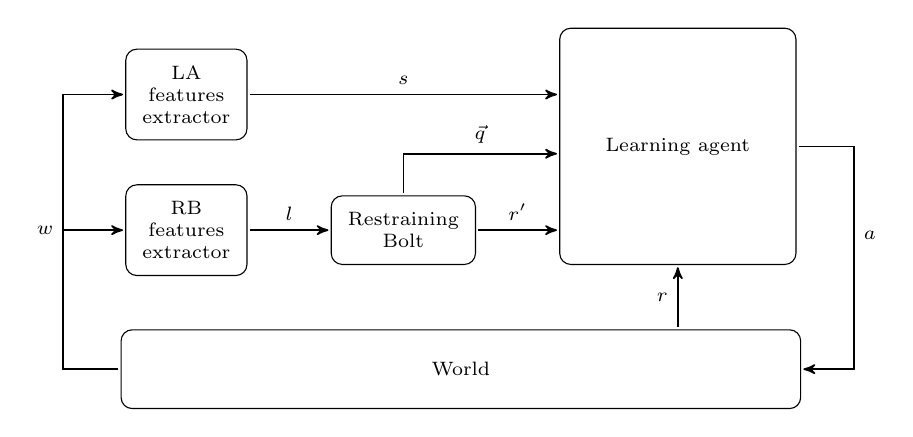
\begin{tikzpicture}[
			every node/.append style={font=\scriptsize},
			arrow/.style={->, semithick},
		]
		\node (rb-features) [block] {RB\\features\\extractor};
		\node (rb) [block, right=of rb-features]  {Restraining\\Bolt};
		\node (agent) [block, right=of rb.south east, anchor=south west,
				minimum width=3cm, minimum height=3cm]
			{Learning agent};
		\node (agent-south) [below=1.2cm of agent.south east, inner sep=0pt] {};
		\node (rb-features-south) [below=1.2cm of rb-features.south west, inner sep=0pt] {};
		\node (world-block) [block, fit=(rb-features-south) (agent-south),
			inner sep=0, minimum height=1cm] {};
		\node at (world-block.center) {\scriptsize World};
		\node (agent-features) [block, above=0.5cm of rb-features]
			{LA\\features\\extractor};
		%
		\draw [arrow] (agent.east) -- +(0.7,0) |-
			node [right, pos=0.2] {$a$} (world-block);
		\coordinate (world-west) at ($(world-block.west)+(-0.7,0)$);
		\node [anchor=east] at (world-west |- rb-features.west) {$w$};
		\draw [arrow] (world-block.west) -- (world-west) |- (rb-features);
		\draw [arrow] (world-west |- rb-features.west) |- (agent-features);
		\draw [arrow] (rb-features) -- node [above] {$l$} (rb);
		\draw [arrow] (rb) -- node [above] {$r'$} (agent.west |- rb.east);
		\draw [arrow] (agent-features) -- node [above] {$s$}
			(agent.west |- agent-features);
		\draw [arrow] (rb.north) -- +(0,0.5) -- node [above] {$\vec{q}$} 
			($(rb.north -| agent.west)+(0,0.5)$);
		\draw [arrow] (world-block.north -| agent.south) --
			node [left] {$r$} (agent.south);
	\end{tikzpicture}
	\caption{Learning agent with Restraining Bolt applied. $r$ is the classic
	MDP reward; $r'$ is the additional non-Markovian reward generated.}
	\label{fig:rb-schema}
\end{figure}
Notice, in particular, that the learning agent has access to the original
observations~$s$ and rewards~$r$, and the additional non-Markovian
rewards~$r'$.  The quantity $\vec{q}$ will be discussed shortly. Let's now
formalize this problem.
\begin{definition}
	\cite{bib:bolt} A \emph{RL problem with \ldl{} restraining specifications}
	is a pair $\langle \mdpS, \const{RB} \rangle$, where: $\mdpS \coloneqq
	\langle S, A, T, R \rangle$ represents a learning agent, and $\const{RB}
	\coloneqq \langle \highlevelS, \set{(\formula_i, r_i')_{i=1}^m} \rangle$ is
	a Restraining Bolt formed by a set of \ldl{} formulae $\formula_i$ over
	$\fluents$ with associated rewards~$r_i'$.
	\label{def:rb-problem}
\end{definition}

We can't simply apply a RL algorithm on the rewards $r_i, r_i'$ over the state
space~$S$, because $r_i'$ are non-Markovian in $S$. What we can do, instead,
is to formulate a NMRDP with \ldl{} rewards, that we already know how to
solve. The complete proof is shown in~\cite{bib:bolt}
and~\cite{bib:favorito-thesis}.	What we see here is a shorter explanation that
just highlights the main concepts.

We first observe that, in Definition~\ref{def:rb-problem}, the MDP and the
Restraining Bolt are completely distinct; their only interaction is in the sum
of the rewards they produce (let's denote with $\bar{r}_i \coloneqq r_i +
r_i'$ the combined reward). So, to simplify the computation, we may keep
these two problems separate, transform the restraining specifications to their
equivalent MDP and combine them later. This is possible because, given two
MDPs, $\mdpS_a = \langle S_a, A, T_a, R_a \rangle$ and $\mdpS_b = \langle S_b,
A, T_b, R_b \rangle$, the following~$\mdpS_{ab} \coloneqq \langle S_{ab}, A,
T_{ab}, R_{ab} \rangle$, with states $S_{ab} \coloneqq S_a \times S_b$,
transition function $T_{ab}: S_{ab} \times A \times S_{ab} \to \R$ and rewards
\[
	R_{ab}((s_a, s_b), a, (s_a', s_b')) \coloneqq R_a(s_{a}, a, s_{a}') +
	R_b(s_{b}, a, s_{b}')
\]
is still an MDP.  Note that we didn't define $T_{ab}$. This is not required,
as in RL, it is sufficient that this unknown function exists; and by the laws
of probability, this is certainly the case, because the existence of $T_a$ and
$T_b$ is a stronger requirement.

Every Restraining Bolt $\const{RB} = \langle \highlevelS, \set{(\formula_i,
r_i')_{i=1}^m} \rangle$ defines a NMRDP with \ldl{} rewards
$\nmrdpS_{\const{RB}} \coloneqq \langle \highlevelS, A, T_\highlevelS,
\set{(\formula_i, r_i')_{i=1}^m} \rangle$, with states $\highlevelS =
2^\fluents$ and $T_\highlevelS$ as the unknown transition function over
fluents configurations. This is a problem that we already know how to solve.
By directly applying Definition~\ref{def:ldlf-eq-mdp}, we can write the
extended MDP~$\mdpS_{\const{RB}} \coloneqq \langle S_{\const{rb}}, A,
T_{\const{rb}}, R_{\const{rb}} \rangle$ that is equivalent to the
NMRDP~$\nmrdpS_{\const{RB}}$. Notice in particular, that the state space
becomes: $S_{\const{rb}} \coloneqq Q_1 \times \dots \times Q_m \times
\highlevelS$, where each $Q_i$ is the set of states of the $i$-th automaton.
For brevity, we will denote elements of $Q_1 \times \dots \times Q_m$ with
$\vec{q}$, because they are vectors of automaton states.

We can now combine the original MDP~$\mdpS$ with the one generated from the
Restraining Bolt~$\mdpS_{\const{RB}}$, just like we've done for $\mdpS_{ab}$,
to obtain a new unified MDP that is defined as $\mdpS' \coloneqq \langle S',
A, T', R' \rangle$, where:
\begin{itemize}
	\item $S' \coloneqq Q_1 \times \dots \times Q_m \times \highlevelS \times S$
	\item $T' : S' \times A \times S' \to \R$ with:
		\begin{multline*}
			T'((q_1, \dots, q_m, l, s), a, (q_1', \dots, q_m', l', s')) \coloneqq \\
			\begin{cases}
				T_{l,s}((l,s), a, (l',s')) &
					\text{if $\forall i : \delta_i(q_i, l') = q_i'$} \\
				0 & \text{otherwise}
			\end{cases}
		\end{multline*}
	\item $R' : S' \times A \times S' \to \R$ with:
		\[
			R'((q_1, \dots, q_m, l, s), a, (q_1', \dots, q_m', l', s')) \coloneqq
			\sum_{i\, :\, q_i' \in F_i} r_i' + R(s, a, s')
		\]
\end{itemize}
Both $T_{l,s}$, that is the joint transition function of the symbols $s$ and
$l$, and the original reward function, $R$, are unknown: we only observe the
samples produced while the agent plays. Instead, we have to move all
automata and return the associated rewards, because this is a dynamics we've
defined.

To this point, we've reduced the original problem of
Definition~\ref{def:rb-problem} to standard RL on the MDP~$\mdpS'$. However,
we can move one step further. In fact, the combined rewards $\bar{r}_i$ do not
depend on the fluents configurations~$l_i \in \highlevelS$, if both $s_i$
and $\vec{q}_i$ are given, that is:
\[
	\bar{r}_t \perp l_0, \dots, l_t \given \vec{q}_t, s_t \qquad
	\text{for any $t$}
\]
This means that an optimal policy exists for $\mdpS'$ with the form:
$\optimal\policy: Q_1 \times \dots \times Q_m \times S \to A$.
To prove it formally, we would need to show that the value of any state
$(\vec{q}, l, s)$, defined in equation~\eqref{eq:mdp-value}, does not depend
on~$l$. We finally get to the following result:
\begin{theorem}
	\cite{bib:bolt} RL with \ldl{} restraining specifications
	$\langle \mdpS, \const{RB} \rangle$, with $\mdpS = \langle S, A, T,
	R \rangle$ and $\const{RB} = \langle \highlevelS, \set{(\formula_i,
	r_i')_{i=1}^m} \rangle$, can be reduced to RL over the MDP $\mdpS'' \coloneqq
	\langle Q_1 \times \dots \times Q_m \times S, A, T'', R''\rangle$,
	and optimal policies for $\langle \mdpS, \const{RB} \rangle$ can be learnt
	by learning corresponding optimal policies for~$\mdpS''$.
	\label{th:bolt-equivalence}
\end{theorem}
If we denote with $S''$ the state space $Q_1 \times \dots \times Q_m \times
S$, the functions $T''$ and $R''$ are partially unknown functions $S'' \times
A \times S'' \to R$, that are defined respectively as $T'$ and $R'$,
marginalized with respect to~$\highlevelS$. With the MDP $\mdpS''$, we assumed
that at each instant $t$, we observe the current state $(\vec{q}_t, s_t)$.
This is true for $s_t$, but not for $\vec{q}_t$. What we can do instead, is
receiving an observation of the symbols $l_t$, moving all the automata
accordingly, and collecting the resulting states~$\vec{q}_t$. So, the new
state $(\vec{q}_t, s_t)$ is composed of the computed vector of automata
states, and the observed symbols~$s_t$. The symbols $\highlevelS$ don't need
to be passed to the learning agent. Refer to Figure~\ref{fig:rb-schema}, once
again.


\subsection{Restraining Bolt for partial observations}

\label{sec:rb-for-partial-obs}

We've thoroughly analyzed solutions for the non-Markovian goals of
Section~\ref{sec:tempoal-goals}: namely, temporally-extended goals. We've
solve them both in isolation, and as additional restraining specifications in
preexisting MDPs. We now want to ask: is it possible to address partial
observations, which is the second source of non-Markovian goals, in a similar
way? In many cases, the answer is yes. Although, as we will see in a moment,
this may not be possible or practical for every problem.

Partially observable environments would be properly modelled with POMDPs
$\langle W, A, T, R, \obsS, O\rangle$, because they define an observation
function $O: W \to \obsS$ that maps world states to observations. However, in
RL, this function is unknown and the states~$W$ are inaccessible for the
agent. So, the simplest approach is to learn a policy directly from the
observation space, $\policy: \obsS \to A$, as if the system were an MDP with
states~$\obsS$ (see Figure~\vref{fig:pomdp-as-mpd}). As we've noted, this can
lead to very poor performances, because rewards can be non-Markovian with
respect to the observations.

Now, let's define a set of fluents~$\fluents$ that represent Boolean
conditions whose truth can be valuated from the observations~$\obsS$.
Similarly to the previous section, to each hidden environment state
corresponds a low-level feature $o \in \obsS$ and a high-level symbol $l \in
2^\fluents$.  In Figure~\ref{fig:symbols-partial-obs}, the environment is
assumed to generate the observation~$o$, on which we have no control. Instead,
the feature extractor indicates that we're free to choose and generate our
high-level alphabet.
\begin{figure}
	\centering
	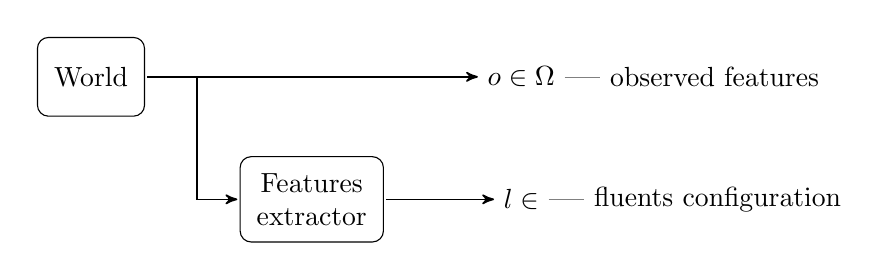
\begin{tikzpicture}[
			arrow/.style={->, semithick},
		]
		\matrix [
			 column sep=1.2cm, row sep=0.5cm,
			] {
			\node (w) [block, minimum height=1cm, minimum width=1cm] {World}; \& \&
			\node (o) [pin=right:observed features] {$o \in \obsS$}; \\ \& 
			\node (f) [block] {Features\\extractor}; \&
			\node (l) [pin=right:fluents configuration] {$l \in \highlevelS$}; \\
		};
		\draw [arrow] (w) -- coordinate [pos=0.15] (inters) (o);
		\draw [arrow] (inters) |- (f);
		\draw [arrow] (f) -- (l);
	\end{tikzpicture}
	\caption{Fluents configurations are computed from observations of the
	environment.}
	\label{fig:symbols-partial-obs}
\end{figure}

Suppose our goal is to define a function that generates the same rewards as
the environment. Since the rewards are non-Markovian with respect to the
observations, they will certainly be non-Markovian with respect to the fluents
configurations which are computed from them. So, what we can do is to define a
NMRDP with \ldl{} rewards from the fluents $\fluents$, that produces the same
rewards~$r$ as the environment. In order to do this, we will certainly select
as fluents all the conditions which are relevant for deciding whether the
reward should be supplied.

\begin{example}
	Let's extend Example~\ref{ex:light}. An agent can control a light bulb
	through a switch, but now it can capture images of the room. Suppose the
	environment rewards the agent with the same condition of the previous
	example: the light must have been switched on, then off, only once during
	the episode.  Our goal is to emulate this reward with a NMRDP with \ldl{}
	rewards.  First, we define a fluent $\const{LightOn}$, representing the
	status of the light. The features extractor, from images of the room in
	which the light is on, would produce $\const{LightOn} = \true$ (or $l =
	\set{\const{LightOn}}$), and false otherwise. Now we state the following
	\ldl{} goal:
	\[
		\formula_1 \coloneqq \ldiamond{(\lnot \const{LightOn})^*;
		\const{LightOn}^+; (\lnot \const{LightOn})^+} \lend
	\]
	where $\resym^+$ is an abbreviation of $\resym; \resym^*$.
	\label{ex:rb-light}
\end{example}

Assuming we've been able to define an NMRDP with \ldl{} rewards, $\nmrdpS =
\langle \highlevelS, A, T, \set{(\formula_i, r_i')_{i=1}^m} \rangle$, that
generates the same rewards as the environment. The equivalent MDP
of~$\nmrdpS$, $\mdpS \coloneqq \langle S', A, T', R' \rangle$ has a state
space $S' \coloneqq Q_1 \times \dots \times Q_m \times \highlevelS$. From
Theorem~\ref{th:bolt-equivalence}, the rewards generated by~$\mdpS$ are the
same as those generated by~$\nmrdpS$.  This also means that the original
rewards, produced by the environment, are Markovian with respect to~$S'$.
Therefore, by augmenting the observations with the automaton states~$\vec{q}$,
we produce a state space that restores the Markov property.  This is possible,
because these states keep track of the unobservable quantities in the
environment state that affect future rewards. This is the important additional
information that we need to provide to the agent, we may even not supply the
rewards that we generate at all. Figure~\ref{fig:rb-partial-obs} shows this
arrangement.
\begin{figure}
	\centering
	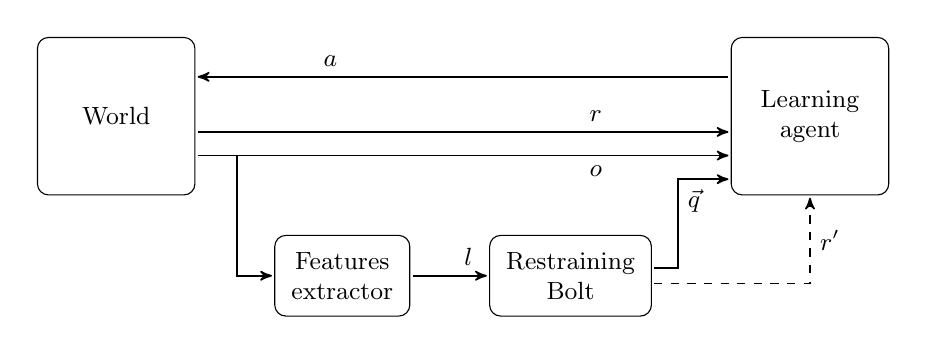
\begin{tikzpicture}[
			every node/.append style={font=\small},
			arrow/.style={->, semithick},
		]
		\matrix [
			 row sep=0.5cm, column sep=1cm,
		] {
			\node (env) [block, minimum size=2cm] {World}; \& \& \&
			\node (agent) [block, minimum size=2cm] {Learning\\agent}; \\
			\&
			\node (features) [block] {Features\\extractor}; \&
			\node (rb) [block] {Restraining\\Bolt}; \& \\
		};
		\coordinate (a1) at ($(agent.west)+(0,0.5)$);
		\draw [arrow] (a1) -- node [near end, above] {$a$} (env.east |- a1);
		\coordinate (w1) at ($(env.east)+(0,-0.2)$);
		\draw [arrow] (w1) -- node [near end, above] {$r$} (agent.west |- w1);
		\coordinate (w2) at ($(env.east)+(0,-0.5)$);
		\draw [arrow] (w2) -- node [near end, below] {$o$} (agent.west |- w2);
		\draw [arrow] (w2) ++(0.5,0) |- (features.west);
		\draw [arrow] (features) -- node [near end, above] {$l$} (rb);
		\draw [arrow] ($(rb.east)+(0,0.1)$) -- ++(0.3,0)
			|- node [below right] {$\vec{q}$} ($(agent.west)+(0,-0.8)$);
		\draw [arrow, dashed] ($(rb.east)+(0,-0.1)$)
			-| node [near end,right] {$r'$} (agent.south);
	\end{tikzpicture}
	\caption{Restraining Bolt for partial observations: RL on the state
	$(o, \vec{q}\,)$.}
	\label{fig:rb-partial-obs}
\end{figure}

\begin{example}
	We now conclude the Example~\ref{ex:rb-light}, where we've prepared an NMRDP
	with a single \ldl{} reward associated to the condition~$\formula_1$. The
	DFA that is associated to this formula is shown in
	Figure~\ref{fig:rb-light-automa}.
	\begin{figure}
			\centering
			\begin{tikzpicture}
			\graph [
				automaton, grow right=3cm,
			]{
				0 ->
					1 [>"$\const{LightOn}$"] ->
					2 [accept,>"$\lnot\const{LightOn}$"] -> ["$\const{LightOn}$"] 3;
				0 -> [self loop above, "$\lnot\const{LightOn}$"] 0;
				1 -> [self loop above] 1;
				2 -> [self loop above] 2;
				3 -> [self loop above, "$\true$"] 3;
			}; 
			\draw [init path] (0.west) +(-0.5,0) -- (0.west);
			\end{tikzpicture} 
			\caption{The DFA associated to the formula~$\formula_1$, in
			Example~\ref{ex:rb-light}.}
			\label{fig:rb-light-automa}
	\end{figure}
	The MDP associated to this simple problem is: $\langle Q \times \obsS, A, T,
	\set{(\formula_1, r')} \rangle$, where the actions are $A \coloneqq
	\set{\const{Toggle}, \const{NoOp}}$, $\obsS$ is an image, and $Q \coloneqq
	\set{0, 1, 2, 3}$. With this composite state space, the agent has a complete
	view about the missing steps to achieve the reward; something that it
	wouldn't know from the current image or the current value of
	$\const{LightOn}$.
	\label{ex:light-rb-automa}
\end{example}

We've previously mentioned that this solution may not be feasible for every
problem. In fact, we must first exclude all environments in which the
observations are not meaningful enough. More precisely, those in which we
cannot accurately predict the next reward~$r_t$ from the sequence of
observations $\langle o_1, \dots, o_t \rangle$. However, these problems would
be problematic for any learning algorithm, due to their weak observation
function. A second group of environments may define reward functions which are
difficult to express in temporal logic. Expressing these goals in \ldl{} would
generate a large number of fluents and obscure temporal specifications
(example: the game of Chess with partial observations of
Example~\ref{ex:chess-partial-obs}). However, this last limitation is not as
strong as it may seem: often, it is possible to greatly simplify the temporal
specification by simply selecting a different set of fluents.

We might think that reproducing the environment's reward function is
impossible if it is unknown. This is not necessarily true, because we are
those that define the agent's goal and would generate those ``environment's''
rewards. For an unknown function, we mean that a precise model of that
function is not available and cannot be exploited, not that the rewarded goal
is obscure. For example, the rewards of Example~\ref{ex:rb-light} are unknown,
because we don't know the function that maps \emph{images} to rewards.


\subsubsection*{Conclusion}

In this Chapter, we've shown that our construction for NMRDP with \ldl{}
rewards, that we call ``Restraining Bolt'', is a valid solution for many
problems: temporally-extended tasks, restraining specifications and partial
observations. A very interesting aspect is that it can be applied as an
additional module, added to the agent's original design. This is possible,
because the extended MDPs only augment the original state spaces with
additional informations. As we will see in the next section, in practice, the
agent requires few modification in order to properly handle these additional
informations. However, the Restraining Bolt is a first important step toward
modularity and explainablility of (Deep) RL agents designed for complex
goals.


% TODO: only reward one. Where to write

\section{Restrained Deep RL agents}

\label{sec:rb-deep-model}

As illustrated in Section~\ref{sec:deep-q-agents}, the RL algorithm used in
this thesis is Double DQN, a Deep RL method. Double DQN agents contain a
Q-Network, which is a function $Q: S \to \R^{\abs{A}}$, that is parametrized
in~$\param$. Given a MDP state~$s \in S$, this computes the state-action
value for every action $a \in A$. In this section, we will propose an original
Q-Network model that properly handles the additional inputs received from the
Restraining Bolt.

The Restraining Bolt is an interesting method because we can regard it as a
module that, added to the original setup, generates additional rewards and
observations. In principle, no structural modifications would be required in
the agent's design: new rewards can be simply summed with the previous ones,
and the Restraining Bolt's states~$\vec{q}$ can be stacked with the
environment's observations to produce a composite MDP state~$(o_t,
\vec{q}_t)$. Agents can learn from this new state space without
modifications\footnote{Extending the size of a table, in order to account for
the additional number of states, is not considered a real modification in the
agent's design.}.

Deep RL agents, instead, learn approximate value functions and policies. In
this case, we should carefully select the agent's model, a neural network,
that has the appropriate expressive power. A network that is suitable to
approximate a function $\obsS \to \R^{\abs{A}}$ is not necessarily appropriate
for a function from the new state space, $\obsS \times Q_1 \times \dots \times
Q_m$. Overfitting and underfitting are well known issues in Machine Learning.


\subsection{Q-Network for the Atari games}

\label{sec:model-atari}

We will first illustrate the agent's model that we use in this thesis when the
Bolt is not applied. Then, in Section~\ref{sec:model-atari-rb}, we'll propose
a modification of this network that accounts for the additional states of the
Restraining Bolt.  The environments used in this thesis are games from the
collection ``Atari~2600''.  As illustrated in Section~\ref{sec:atari-envs},
the observations produced are frames of size $(210, 160)$, with an RGB colour
depth of 8-bit. Each game defines a different number of actions, 18 at most.

We use the same architecture as~\cite{bib:atari-deepq-nature}, which is
illustrated here. Slight modifications will be listed in the implementation
part, in Section~\ref{sec:impl-agent}. First, a preprocessing function applies
a fixed transformation to each image. Every frame is converted to a gray-scale
picture, by computing the luminance value of each pixel. The image is then
resized to $(84, 84)$, in order to reduce the input dimensionality. Finally, 4
consecutive images are combined together, producing a tensor of size $(84, 84,
4)$ that can be passed to the network. This last combination allows to create
an observation that encodes how the objects in the scene are moving. The lack
of this information is one of the causes of non-Markovian rewards that can be
easily solved. See Example~\ref{ex:motion}, for an explanation.

Let's define the following abbreviation: \convlayer{$n$}{$s$}{$t$} represents
a 2D convolutional layer composed of a number of $n$ filters of size $s \times
s$ with a stride of $t$. Similarly, \denselayer{$n$} represents a
fully-connected layer of $n$ units. We can now define the network structure
as:
\begin{center}
	\convlayer{32}{8}{4}, \relu{}, \\
	\convlayer{64}{4}{2}, \relu{}, \\
	\convlayer{64}{3}{1}, \relu{}, \\
	\denselayer{512}, \relu{}, \\
	\denselayer{$\abs{A}$}
\end{center}
where \relu{} is the rectifier linear unit applied to each element. In neural
networks, images are frequently transformed with a cascade of 2D convolutions,
followed by a number of dense layers. The authors of the original
paper~\cite{bib:atari-deepq-nature} have shown that this network size
generates a model with the appropriate expressive power for our environments.


\subsection{Q-Network for the Restraining Bolt}

\label{sec:model-atari-rb}

We now want to apply the method presented in
Section~\ref{sec:rb-for-partial-obs} in those games in which low performances
are caused by partial observations. This means that our agent would need to
receive the original observation, which is a frame of the game, and the
vector of the Bolt's states,~$\vec{q}$. We'll now suppose that our
temporally-extended goal can be expressed with a single pair ${(\formula,
r')}$. So, the Restraining Bolt's state is a single scalar identifier~$q$.

As anticipated, we cannot simply stack $o$ and $q$. Even if the network
architecture would allow that, we would assign a very low relative importance
to $q$ among the thousands of pixels of which $o$ is composed. Most
importantly, the role of $q$ must not be confused with pixels. All these
considerations are important because every model introduces some biases, and
we want our model's bias to capture the following basic intuition: $q$ is an
important index that parametrizes value functions. The state $q$ is a
parametrization over value functions because, to different automaton states,
there may correspond dramatically different value functions over inputs.

\begin{example}
	Let's consider again the light bulb of Example~\ref{ex:light-rb-automa} and
	the automaton of Figure~\ref{fig:rb-light-automa}. Suppose the initial MDP
	state is $s_0 = (o_0, 0)$, where $o_0$ is an image of a dark room. In this
	case, the model should learn an high state-action value for the action
	$\const{Toggle}$, and a low value for the action $\const{NoOp}$. Later on,
	at some time~$t$, the agent may observe the following input: $s_t = (o_0,
	2)$. Even though the image is the same, the agent should assign the highest
	value to $\const{NoOp}$. A different automaton state dramatically changes
	the most promising actions that will lead to the goal.
\end{example}

A very drastic choice would be to maintain a number of $\abs{Q}$ different
networks, with the same architecture but different parameters~$\param_1,
\dots, \param_{\abs{Q}}$. At each step, given an input $(o, q)$ the agent may
use the network $\param_q$ to predict the actions values for the input~$o$.
This strong parametrization would completely separate the value functions.
An immediate problem with this approach is space inefficiency (that would be
very evident with large $Q$ or vectorial~$\vec{q}$). Most importantly, the
networks associated to states that are rarely encountered would be trained
on too few input samples.

The model that we propose here is a variant of the network of the previous
section. We substitute the last fully-connected layer with one of dimension
$\abs{A} \times \abs{Q}$. This means that a number of $\abs{A} \cdot \abs{Q}$
linear units is arranged as a matrix, whose first index is an action and
the second index is a Bolt's state. So, for each automaton state, the net will
generate a different column of state-action values. The idea behind this
choice is that we can safely share the initial layers, whose main goal is to
provide an encoding of the observed input. Instead, separating the last layer
provides the greatest flexibility among other combinations\footnote{
	We didn't motivate why the first layers of the original net should behave as
	an encoder. However, after the modification, they will be shared and trained
	with different outputs. So, this role will be encouraged.
}. This is an intermediate approach between completely shared and completely
separate parameters~$\param_1, \dots, \param_{\abs{Q}}$. For a
vectorial~$\vec{q}$, it can be easily extended: the last fully-connected layer
would produce tensors of shape $(\abs{A} \times \abs{Q_1} \times \dots \times
\abs{Q_m})$. Since the greatest number of parameters is shared, each
combination of automaton states $\vec{q}$ requires a smaller number of
training samples to train on.

The resulting Q-Network for the Atari games is:
\begin{center}
	\convlayer{32}{8}{4}, \relu{}, \\
	\convlayer{64}{4}{2}, \relu{}, \\
	\convlayer{64}{3}{1}, \relu{}, \\
	\denselayer{512}, \relu{}, \\
	\denselayer{$\abs{A} \times \abs{Q}$}, \\
	\slicelayer{$\cdot, q$}
\end{center}
where \slicelayer{$\cdot, q$} indicates that we select the $q$-th column of
the input matrix. This is the agent's model used in this thesis. As we can
see, we didn't need to define more than one temporal goal in our experiments.

Some other variants may exists. In fact, we should remember that the automata
states are generated from the conversion of  \ldl{} or \ltl{} expressions.
Since, this translation has a worst case complexity that is doubly exponential
in the size of the formula, the state space may be quite large. One
possibility would be to investigate whether is it possible to adopt the NFA
states, instead of the DFA's, producing a state space that may be
exponentially smaller (multiple columns would be active at the same time, in
this case). But these variants have not been investigated yet.

\chapter{Learning to valuate fluents in games}

The importance of correctly valuate the fluents.

\section{Temporal constraints}

How we can use temporal logic to express legal traces of interpretations;
e.g. expected behaviours.

\section{Assumptions}

A temporal constraints aren't definitions; they are just minimal constraints.
We need additional clues: visual description of fluents.
Now follow my assumptions:
\begin{itemize}
	\item Local propertes (with regions I don't have to find elements in a
		frame).
	\item The property is visually apparent, inside the region.
\end{itemize}

Limitations and other ideas for a stronger grouding.

\section{General structure of the model}

Illustration and general description of the model.

\section{Encoding}

Encoder: the model, how it works, what does it learn, size of the encoding.

References:
Training Restricted Boltzmann Machines and Deep Belief Neworks
\cite{bib:rbm-training}\cite{bib:ml-book-murphy}.

\subsection{Model: Deep Belief Network}

\subsection{What does it learn}


\section{Boolean functions}

The fluents are true in a set of those configurations.

\subsection{Learning with genetic algorithms}

Ideas from concept learning; genetic algorithm.

References:
Genetic Algorithms for Concept learning\cite{bib:ga-for-concepts},
Genetic Algorithms review\cite{bib:ga-mutations-review}.

\subsection{Boolean rules}

Representation of boolean functions and training details.

\chapter{AtariEyes package}

\label{ch:atarieyes}

This chapter describes the software realized in this thesis, that we called
``AtariEyes''. Its purpose is both to implement the ideas that have been
presented in previous chapters and to generate the experiments shown
Chapter~\ref{ch:experiments}.

Apart from being a realization of the ideas proposed, this software has some
interesting qualities:
\begin{description}
	\item [Clarity] Every method and structure has been documented.
	\item [Efficiency] Thanks to an heavy use of parallel computing libraries,
		it benefits from GPU acceleration.
	\item [User friendly] The extensive command line interface allows to
		experiment with the package as it is, or, thanks to its modular design,
		individual structures can be reused in future developments.
\end{description}

Regarding its general functionality, through the commands provided, the user
can:
\begin{itemize}
	\item Choose any \emph{environment} from the Atari~2600 collection.
	\item Train a Deep Reinforcement Learning \emph{agent}. The algorithm is
		Double DQN and the agent's model can be either the original Atari model
		(Section~\ref{sec:model-atari}) or the restricted agent
		(Section~\ref{sec:model-atari-rb}).
	\item Train the \emph{feature extractor}, because it implements every model
		and algorithm presented in Chapter~\ref{ch:fluents}.
	\item \emph{Play}, \emph{visualize} and \emph{record} any of these
		agents while they interact with the environment.
\end{itemize}

This chapter is divided in two sections: Section~\ref{sec:how-to-use}
documents how the software can be used from a user perspective;
Section~\ref{sec:implementation} is a larger part that explains some of the
most interesting details about the implementation.
%While the former is really
%useful for an high-level overview, the latter highlights some interesting
%parts which may be useful also in future developments.


\section{How to use the software}

\label{sec:how-to-use}

\subsection{Tools and setup}

The software \texttt{AtariEyes} is a Python package. It is publicly available
at the GitHub repository:
\href{https://github.com/cipollone/atarieyes}{\texttt{cipollone/atarieyes}}.
It can be installed with the \texttt{pip} commandAs any other Python package,
we just need to point to this git repository. The installation
command is:
\begin{minted}{text}
pip install git+https://github.com/cipollone/atarieyes
\end{minted}
This installs this package from the master branch. If we need to work on some
specific revision, for example on the \texttt{develop} branch, we can append
\verb!@develop! or any other commit to the previous address.

Dependencies are automatically installed by \texttt{pip}.  In Python, it is
common to run applications inside virtual environments. Just run this
installation command within a container to avoid dependency conflicts with
other applications. One rather particular dependency is TensorFlow, which is a
famous Machine Learning library that we use for parallel computing. Following
the instructions of the specific container application, we can reuse some
preexisting system installation, if we need. Currently, the supported version
is only 2.1, but future 2.x versions might also be compatible.

The package is written in Python~3 and the minimum version required for the
interpreter is 3.7. This requirement should be met by most modern operating
systems. If that's not the case, we suggest to use \texttt{pyenv}, which
allows environment-specific Python installations.

Once installed, we can use the \texttt{atarieyes} package. As we will see, we
often use this module through its command line interface. However, if we want
just to include some structures and algorithms in other applications, we can
\mintinline{py3}|import atarieyes|, as usual. For development it may
be also useful to look at the source code. We can clone the repository:
\begin{minted}{text}
git clone https://github.com/cipollone/atarieyes.git
\end{minted}
This is also useful if, for any reason, some updated dependency is no longer
compatible with this package. What we can do is to \texttt{cd} to this cloned
directory, then run \texttt{poetry install}. Poetry is the container
application that we use. This command will install the exact dependency
versions that have been used during development and are guaranteed to work.


\subsection{Execution}

To run this package as a script we run the following command from the same
environment where we've installed it:
\begin{minted}{text}
python3 -m atarieyes
\end{minted}
The reader can assume that any \texttt{atarieyes} command that we will see, is
executed by \verb|python3 -m|.

\subsubsection*{Getting help}

The package provides a compete command line interface, with many options that
control the training process. In these sections we look at the most important
commands. For any doubt, we can use the \verb|--help| option, abbreviated
as \verb|-h|. When added, it prints the arguments that are supported by any
command. For example, running \verb|atarieyes -h|
produces the following message\footnote{We use the
\texttt{argparse} library for parsing and generating these messages. The file
\texttt{\_\_main\_\_.py} file also acts as reference for the commands.}:
\begin{minted}{text}
usage: __main__.py [-h] [--list] [--from FROM] {agent,features} ...

Feature extraction and RL on Atari Games

positional arguments:
  {agent,features}  Choose group
    agent           Reinforcement Learning agent
    features        Features extraction

optional arguments:
  -h, --help        show this help message and exit
  --list            List all environments, then exit
  --from FROM       Load arguments from file
\end{minted}

The \verb|--list| option prints the unique of every Atari game. To use any of
these games as environment, we pass its identifier to the
\verb|--env|/\texttt{-e} option, where appropriate.

The \verb|--from| option allows to execute the command and options stored some
JSON file. The JSON must be a dictionary of pairs: argument name--argument
value. The interface of this file is exactly the same of the command line
interface that we're describing. After any ``train'' command, an
\verb|args.json| is automatically saved. The purpose of this option is
allowing to repeat, resume or slightly modify a command that was previously
used.

All commands are divided in two groups. The \texttt{agent} commands regard the
RL agent, while \texttt{features} commands are related to the features
extractor.


\subsubsection*{Agents}

Three operations can be performed for the agent: \texttt{train},
\texttt{play}, and \texttt{watch}.

To train an agent we run:
\begin{minted}[escapeinside=||]{bash}
atarieyes agent train      # ...
\end{minted}
This command has many options, some of which control the parameters of the
Double DQN algorithm. We show here just the most relevant:
\begin{description}
	\item [\texttt{-e}/\texttt{--env}] Selects the environment to use among the
		list of Atari games.
	\item [\texttt{-b}/\texttt{--batch}] Each update of the Q-Network is
		computed from a cumulative gradient of this number of samples.
	\item [\texttt{-r}/\texttt{--rate}] Chooses the learning rate associated
		to each gradient update.
	\item [\texttt{-g}/\texttt{--gamma}] Selects a discount factor.
	\item [\texttt{-c}/\texttt{--continue}] Resumes training from any
		checkpoint. Checkpoints are saved in regular intervals, according to the
		\texttt{--save} option, or when a training is interrupted with CTRL-C
		(SIGINT).
	\item [\texttt{--rb}] Trains an agent with the Restraining Bolt applied.
		When this option is absent, the agent Q-Network is that of
		Section~\ref{sec:model-atari}. When \texttt{--rb} is added, the
		restrained model from Section~\ref{sec:model-atari-rb} is used.
		The argument of this command is the IP of a running Restraining Bolt;
		often, just \texttt{localhost}.
\end{description}
There are many other options which we didn't list here.

The second command related to agents is \texttt{play}. Its purpose is to load
an agent previously trained and let it interact with the environment. This is
certainly useful to assess the performances reached. Most importantly, this
continuous play generates the stream of observations that we need in order to
train a features extractor. Some options are:
\begin{description}
	\item [\texttt{args\_file}] This mandatory argument is the path of the JSON
		file containing the exact training command of the agent.
	\item [\texttt{-c}/\texttt{--continue}] It is a mandatory argument that
		says which checkpoint to load.
	\item [\texttt{--rand-eps} {\normalfont and} \texttt{--explore-policy}]
		These two options allow to use the two custom exploration policies that
		were defined in Section~\ref{sec:exploration-policies}.
	\item [\texttt{-w}/\texttt{--watch}] To visualize the frames of the game.
		Allowed arguments are \texttt{render}, to watch the images on screen while
		the agent plays, or \texttt{stream} to send them to another running
		instance. These can be received by another instance training the
		features extractor model.
	\item [\texttt{--record}] To save a video of the agent's performance.
\end{description}


\subsubsection*{Features}

Commands that start with \texttt{atarieyes features} are related to the
features extractor. We can train the model that was developed in
Chapter~\ref{ch:fluents} and use it for prediction withing a
Restraining Bolt.

The first step is to define a set of fluents to learn, and their associated
regions. The \texttt{select} command allows to easily select the regions for
an environment. For example, to define regions in the Pong game, we run:
\begin{minted}{text}
atarieyes features select -e Pong-v4
\end{minted}
where \texttt{Pong-v4} is the precise name of the environment. After this
command, a frame of the game is shown. With the mouse we can do one or more
selections (press Enter to accept). The first selection is the portion of the
image where the agent should be trained (allowing to cut irrelevant parts).
Then, every following selection is a definition of a new region. After each
selection we insert at the terminal an unique name and abbreviation for that
region.

The output generated is a JSON file containing our definitions that we can now
modify and integrate. We could have written this file manually, but
\texttt{select} is a convenient way to start. The file is saved at
\texttt{definitions/}<env-name>\texttt{.json}. In our example on the Pong
environment, the output is shown in Listing~\ref{lst:pong-def-example}
\begin{listing}
\begin{minted}{json}
{
  "_frame": [ 0, 33, 160, 195 ],
  "regions": {
    "paddle_right": {
      "abbrev": "pr",
      "region": [ 131, 34, 151, 196 ],
      "fluents": []
    },
    "bottom": {
      "abbrev": "bot",
      "region": [ 0, 184, 160, 194 ],
      "fluents": []
    }
  },
  "constraints": [],
  "restraining_bolt": []
}
\end{minted}
\caption{Example for the Pong game; file \texttt{definitions/Pong-v4.json}}
\label{lst:pong-def-example}
\end{listing}
which lists each region name, abbreviation, coordinates, and fluents defined.
Now we can fill each \verb|"fluents"| with the list of symbols that we want to
define in that region.

The other two empty fields are \verb|"constraints"| and
\verb|"restraining_bolt"|. Here we write the \ldl{} formulae for the temporal
constraints (Section~\ref{sec:temporal-constraints}) and for the Restraining
Bolt temporal specification (Section~\ref{sec:rb}), respectively. The atomic
symbols of both formulae must be among the fluents we've defined above. In
this file, they are stored as lists just to improve readability. All
expressions each list are joined through conjunction in a single \ldl{}
formula. Since the \texttt{constraints} are always satisfied, we consider as
restraining specification the conjunction of both fields.

After the definitions, we're ready to train the valuation functions.
This is achieved by the \verb|atarieyes features train|, much
like we've done for the agent. Few of the many options of this command are:
\begin{description}
	\item [\texttt{--stream}] Sets the IP address of a running instance of
		\verb|agent play --watch stream| (default is \texttt{localhost}). The
		frames received are used to train this model.
	\item [\texttt{--shuffle}] Sets the size of the dataset composed by the most
		recent observations.
	\item [\texttt{-c}/\texttt{--continue}] Resumes an interrupted training from 
		a checkpoint.
	\item [\texttt{-i}/\texttt{--init}] Starts a new training but initializes
		the parameters from a checkpoint.
	\item [\texttt{--train}] The two arguments that follow are the name and the
		depth of the layer that should be trained by this command. Other parts of
		the model are not modified.
	\item [\texttt{--network}] Specifies the structure of the encoders. The
		argument of this command is a list of natural numbers. The $i$-th number
		indicates of how many hidden units is composed the $i$-th layer of each
		DBN.
\end{description}
The features extractor that we've defined in Chapter~\ref{ch:fluents} is
composed by one DBN for each region (the encoders) and the Boolean functions,
shared by all regions. The encoders, in turn, contain a stack of RBMs, which
are organized in layers. For each region, we need to train the shallow layers
first. For example as:
\begin{minted}{text}
atarieyes features train -e Pong-v4 --network 20 3 --train bottom 0
\end{minted}
Then, we proceed to the next layer just below (in this example,
\verb|bottom 1| is the next and last layer of this encoder). After each
encoder is trained, we can proceed to train the Boolean functions with
\verb|--train all -1|. Each time we proceed to a different part of the model,
we should initialize the parameters from the previous result via the
\texttt{--init} option.

Many other options, which we didn't list here, allow to personalize both
Persistent CD and the Genetic Algorithm. For example, we can tune how many
episodes are executed when computing the fitness function.

Once every part of the features extractor is trained, we can use it to make
predictions. In particular, we pass the predicted fluents values to the
Restraining Bolt. With the command \texttt{features rb} we can execute a RB
from the features extractor just trained. Some arguments are:
\begin{description}
	\item [\texttt{args\_file}] Mandatory path of the JSON file of arguments
		that generated the features extractor.
	\item [\texttt{-i}/\texttt{--init}] Model checkpoint to load.
	\item [\texttt{--stream}] IP address of the running agent to which this
		Restraining Bolt should be applied.
\end{description}


\subsubsection*{Instances}

As we can understand from the arguments of the various commands, often we need
to run more than one instance at the time. Figure~\ref{fig:cmd-instances}
shows how the instances interact in each situation.

\begin{figure}[p]
	\centering
	\subfloat[][Training a features extractor.] {
	\begin{tikzpicture}
		\node (play) [command text] {
			atarieyes agent play {\normalfont <agent-file>} --watch stream
		};
		\node (train) [command text, below=1.5cm of play] {
			atarieyes features train --env {\normalfont <env-name>}
		};
		\draw [flow] (play) -- node (mid) [midway] {} (train);
		\coordinate (frames) at ($(mid) + (1,0)$);
		\node [anchor=east, outer sep=1ex] at (mid) {$\bvec{o}_t$};
		\node [image, xshift=-0.2cm, yshift=0.2cm, opacity=0.3] at (frames)
			{\includegraphics[width=0.8cm]{./imgs/si0.png}};
		\node [image, xshift=-0.1cm, yshift=0.1cm, opacity=0.6] at (frames)
			{\includegraphics[width=0.8cm]{./imgs/si0.png}};
		\node [image] at (frames)
			{\includegraphics[width=0.8cm]{./imgs/si0.png}};
		%
		\begin{pgfonlayer}{below}
			\node [fit=(play) (train), box=orange, tight, opacity=0.5] {};
		\end{pgfonlayer}
	\end{tikzpicture}
	} \\[1.5cm]
	\subfloat[][Training a restrained agent.] {
	\begin{tikzpicture}
		\node (rb) [command text] {
			atarieyes features rb {\normalfont <features-file>} --stream
		};
		\node (train) [command text, below=1.5cm of rb] {
			atarieyes agent train --env {\normalfont <env-name>} --rb
		};
		\draw [flow] ([xshift=-2cm]train.north) --
			node (mid) [midway] {} ([xshift=-2cm]rb.south);
		\node [anchor=east, outer sep=1ex] at (mid) {$\bvec{o}_t$};
		\coordinate (frames) at ($(mid) + (1,0)$);
		\node [image, xshift=-0.2cm, yshift=0.2cm, opacity=0.3] at (frames)
			{\includegraphics[width=0.8cm]{./imgs/si0.png}};
		\node [image, xshift=-0.1cm, yshift=0.1cm, opacity=0.6] at (frames)
			{\includegraphics[width=0.8cm]{./imgs/si0.png}};
		\node [image] at (frames)
			{\includegraphics[width=0.8cm]{./imgs/si0.png}};
		\draw [flow] ([xshift=2cm]rb.south) --
			node [anchor=west, outer sep=1ex] {$(\vec{q}_t, r_t')$}
			([xshift=2cm]train.north);
		%
		\begin{pgfonlayer}{below}
			\node [fit=(rb) (train), box=blue!50!lightgray, tight, opacity=0.5] {};
		\end{pgfonlayer}
	\end{tikzpicture}
	} \\[1.5cm]
	\subfloat[][Training a new features extractor from a restrained agent.] {
	\begin{tikzpicture}
		\node (rb) [command text] {
			atarieyes features rb {\normalfont <features-file>} --stream
		};
		\node (play) [command text, below=1.5cm of rb] {
			atarieyes agent play {\normalfont <agent-file>} --rb --watch stream
		};
		\node (train) [command text, below=1.5cm of play] {
			atarieyes features train --env {\normalfont <env-name>}
		};
		\draw [flow] ([xshift=-2cm]play.north) --
			node (mid) [midway] {} ([xshift=-2cm]rb.south);
		\node [anchor=east, outer sep=1ex] at (mid) {$\bvec{o}_t$};
		\coordinate (frames) at ($(mid) + (1,0)$);
		\node [image, xshift=-0.2cm, yshift=0.2cm, opacity=0.3] at (frames)
			{\includegraphics[width=0.8cm]{./imgs/si0.png}};
		\node [image, xshift=-0.1cm, yshift=0.1cm, opacity=0.6] at (frames)
			{\includegraphics[width=0.8cm]{./imgs/si0.png}};
		\node [image] at (frames)
			{\includegraphics[width=0.8cm]{./imgs/si0.png}};
		\draw [flow] ([xshift=2cm]rb.south) --
			node [anchor=west, outer sep=1ex] {$(\vec{q}_t, r_t')$}
			([xshift=2cm]play.north);
		%
		\draw [flow] (play) -- node (mid1) [midway] {} (train);
		\coordinate (frames) at ($(mid1) + (1,0)$);
		\node [anchor=east, outer sep=1ex] at (mid1) {$\bvec{o}_t$};
		\node [image, xshift=-0.2cm, yshift=0.2cm, opacity=0.3] at (frames)
			{\includegraphics[width=0.8cm]{./imgs/si0.png}};
		\node [image, xshift=-0.1cm, yshift=0.1cm, opacity=0.6] at (frames)
			{\includegraphics[width=0.8cm]{./imgs/si0.png}};
		\node [image] at (frames)
			{\includegraphics[width=0.8cm]{./imgs/si0.png}};
		%
		\begin{pgfonlayer}{below}
			\node [fit=(play) (train), box=orange, tight, opacity=0.5] {};
			\node [fit=(rb) (play), box=blue!50!lightgray, tight,
				opacity=0.5] {};
		\end{pgfonlayer}
	\end{tikzpicture}
	}
	\caption{How the various instances interact in each case.}
	\label{fig:cmd-instances}
\end{figure}

These instances use sockets to exchange observations, states and rewards. The
reason for this complete separation is that the main purpose of the
\texttt{atarieyes} package is to implement the Restraining Bolt and the
features extractor of Chapter~\ref{ch:fluents}, not a RL agent. In fact, there
are many modern and stable libraries implementing Deep RL agents. Thanks to
this separation, we can substitute \texttt{atarieyes agent} commands with any
software implementing a Deep RL agent. We don't need to restrict ourselves to
our implementation, not even to Double DQN. In fact, it's sufficient that the
agent's instance respects the interface of the socket messages. Since we also
provide Client--Server classes, the integration should be immediate.


\subsubsection*{Output}

To conclude this overview of the user interface, we look at the output of the 
various commands. As we've seen from \texttt{select}, the definitions for each
environment are stored in JSON files inside the \texttt{definitions/}
directory. Training commands, instead, store their result inside
\texttt{runs/}. For example,
\verb|atarieyes agent train -e Pong-v4| 
generates the following directories:
\begin{minted}{text}
runs/agent/Pong-v4/logs/0/
runs/agent/Pong-v4/models/0/
\end{minted}
Every training generates ``logs'' and ``models'' directories in
unique paths composed with increasing numbers. In the example above, a new
output would be saved \verb|logs/1| and \verb|models/1|.

Inside the ``models'' directory we can find all the checkpoints saved
during training. These files can be passed as arguments to a \verb|--continue|
option, to load a saved agent. ``logs'' directory, instead, contains
\verb|args.json| and a file of TensorBoard logs. The JSON of arguments
\verb|args.json| is used for the \texttt{play} command or for the
\verb|--from| option, if we want to repeat a similar training.

The remaining files in the logs directory contain various metrics that allow
to follow the training process. These logs can be visualized with TensorBoard,
the TensorFlow visualization tool. In the example, we would run:
\begin{minted}{text}
poetry run tensorboard --logdir runs/agent/Pong-v4/logs/
\end{minted}
For each episode, we can read: the number of steps, the cumulative reward, the
distribution of RB states, the distribution of selected actions, and other
metrics related to DQN.

The output of a \texttt{features train} command is really similar to that for
the agent: ``logs'' and ``models'' directories are saved under
\verb|runs/features| that contain the JSON of arguments, checkpoint files, and
TensorBoard logs. Intead, the main difference is the content of the log files.
Some informations that we save and can be visualized are the following:
\begin{description}
	\item [Scalar metrics] These are relevant scalar quantities that allow to
		follow the training algorithm. For RBM training, we store: free energy,
		reconstruction error, sparsity and normalization loss, learning rate.
		Instead, for the Boolean functions, we can read: average and maximum
		values of the sensitivity, consistency metrics, and fitness.
	\item [Images] Reconstructed most probable input images.
	\item [Graph] We can inspect the graph of computation of each step of the
		training algorithm. Each inner model of the features extractor has a
		different training graph. For the Boolean functions, for example, we
		observe the four steps of the genetic algorithm.
	\item [Distributions] We can observe how the model parameters are
		distributed on the real axis. This helps to investigate under/over-fitting
		and other issues. For the genetic algorithm we visualize the population
		fitness values, a projected representation of the individuals, and the
		fluents predictions.
\end{description}


\subsubsection*{\ldl{} library: \texttt{flloat}}

Temporal logic is used for two purposes: the RB restraining specification,
which indicates the agent's behaviour to reward, and the temporal constraint,
used to learn the valuation functions. They are \ldl{} formulae, written
inside each environment JSON file of definitions.

The library that we use for parsing and transforming these formulae to DFA is
called \texttt{flloat} (GitHub \href{https://github.com/whitemech/flloat}{%
\texttt{whitemech/flloat}}). The purpose of the package is to
implement the DFA transformation for two temporal logics: \ltl{} and \ldl{}.
In fact, we might alternatively use \ltl{} with minor modifications to the
source.

The initial author of this library, Favorito~\cite{bib:favorito-thesis},
started this project as a Python port of an homonymous software that was
developed in Java\footnote{GitHub
\href{https://github.com/RiccardoDeMasellis/FLLOAT}{%
\texttt{RiccardoDeMasellis/FLLOAT.}}}. Then, development has continued and,
during this thesis work, we contributed to the advancements of the
library. We helped to improve the overall stability of the software and to
write a more efficient parsing of the input languages (we use version~0.3.0).

The fields \verb|constraints| and \verb|restraining_bolt| both contain \ldl{}
expressions in a string format accepted by \texttt{flloat}.  We can refer to
this library documentation to understand what is format accepted. Since
\texttt{flloat} gets installed with \texttt{atarieyes}, we can also experiment
interactively with it.  For example:
\begin{minted}{py3}
from flloat.parser.ldlf import LDLfParser as Parser

expression = "A & [true*; A]B & <true*; ?B>tt"
formula = Parser()(expression)
automa = formula.to_automaton()
\end{minted}
This is useful to check that the \texttt{expression} has the correct syntax,
and that it represents the intended temporal property (it's possible to
visualize the automaton \texttt{automa} with Graphviz). In this example,
\texttt{expression} is correctly parsed as:
\[
	A \land \lbox{\true^*; A}B \land \ldiamond{\true^*; B?} \ltt
\]



\section{Implementation}

\label{sec:implementation}

The package has a modular and comprehensible design, as we can see from the
following file structure: \\[1ex]
\hspace{2ex}
\begin{minipage}[t]{0.25\textwidth}
	\begin{forest}
		dirtree
		[atarieyes/,baseline
			[\_\_main\_\_]
			[tools]
			[streaming]
			[layers]
			[automata]
		]
	\end{forest}
\end{minipage}
\hfill
\begin{minipage}[t]{0.25\textwidth}
	\begin{forest}
		dirtree
		[atarieyes/,baseline
			[agent/
				[training]
				[playing]
				[models]
			]
		]
	\end{forest}
\end{minipage}
\hfill
\begin{minipage}[t]{0.25\textwidth}
	\begin{forest}
		dirtree
		[atarieyes/,baseline
			[features/
				[training]
				[rb]
				[models]
				[genetic]
				[temporal]
				[selector]
			]
		]
	\end{forest}
\end{minipage}
\vspace{2ex}

\noindent
Each of these files is an importable Python module (extension omitted), with a
separate functionality. We won't discuss all of them, as we only want to look
at the most interesting details of the software.


\subsection{\texttt{atarieyes} package}

There are 5 modules inside the outer scope (left column of the file hierarchy
above). \verb|__main__.py| only realizes the command line interface and
\verb|tools.py| contains generic utilities. Instead, the remaining modules are
the most interesting.


\subsubsection*{\texttt{streaming} module}

This module allows the various instances of the program to communicate. It
defines a communication protocol and the format of the messages to exchange.
The instances communicate through sockets. So, the RL agent and the
Restraining Bolt could even be on separate machines. Furthermore, this allows
our implementation of the features extractor and the Restraining Bolt to
communicate with any kind of RL agent, even implemented with some other
library. It's sufficient that the agent program does
\mintinline{py3}|import atarieyes.streaming| to use this module
interface for exchanging messages with the Restraining Bolt.

This file defines two base classes: \texttt{Sender} and \texttt{Receiver}.
The sender is a TCP server that waits for an incoming connection from the
receiver. They only realize the basic functionality, because the specific
messages format is defined in subclasses.

\texttt{AtariFramesSender} and \texttt{AtariFramesReceiver} is a pair of
subclasses that are used to send images of the Atari games when the
\verb|--stream| option is present. Similarly, \texttt{StateRewardSender} and
\texttt{StateRewardReceiver} transmit the pair $(\vec{q}, r')$ of automaton
state and reward from the RB back to the agent.

Users can send and receive data with \texttt{send} and \texttt{receive}
methods of the respective instances in each pair.  The base classes also
provide transmit and receive buffers for an asynchronous exchange. 


\subsubsection*{\texttt{automata} module}

This module only contains one class that realizes a DFA. There are many
automata libraries available. The motivation behind this class is that we need
to be very efficient in our specific use case: running many copies of the same
automaton. In the following, let's denote with $\automa_\constraintS$ the
DFA associated to the temporal constraint.

The final layer of the features extractor model is composed by an array of
Boolean functions. As we've seen, this part is trained with a Genetic
Algorithm, which maintains a population of candidates (each individual is an
array of functions). Computing the fitness function for each individual
requires to do predictions with all of them and check the generated traces
against the temporal constraint. To do so, we continuously predict the fluents
values with each candidate, and we move each copy of $\automa_\constraintS$
accordingly. At the end of the episodes we combine the metrics to compute the
total fitness function for each candidate. Since the population can contain
thousands of candidates, it's important to have an implementation that allows
an efficient execution of thousands of parallel copies of the same DFA. 

The class \texttt{TfSymbolicAutomaton} stores the edges of the graph into a
Hash table. Each key is a pair containing the current state and the input
symbol; each value is the next state for that key. Moving through the
automaton is a simple lookup from this table. To realize both the table and
the lookup mechanism we've used the vectorial calculus of the TensorFlow
library. So, with just one call, it's possible to receive the next states for
any number of state--symbol input pairs.

The methods are:
\begin{minted}{py3}
def initial_states(self, n_instances): # ...

def is_final(self, states): # ...

def successors(self, states, symbols):
	# Lookup
	keys = self._to_keys(states, symbols)
	next_states = self.transitions.lookup(keys)
	
	return next_states
\end{minted}
The automaton instance is state-less. The caller should maintain a vector of
states, created from \verb|initial_states| and transformed each time with
\texttt{successors}.

The input \texttt{symbols} is a vector of predictions, one for each candidate.
The symbols alphabet is the set of Boolean interpretations of the fluents.
This means that the space occupied by the lookup table is exponential in the
number of fluents. This is not an issue, because the \ldl{} to DFA conversion
has a double-exponential time cost, which is often a much stronger requirement
on the number of usable fluents.


\subsubsection*{\texttt{layers} module}

In Keras, TensorFlow and any modern library, Neural Networks are implemented
as a composition of layers. Although we're not required to use layers, they
allow a better organization of our models. This module defines the basic
functionality related to layers and the specific definitions of layers that
will be used in our networks.

\texttt{BaseLayer} is the base class of any layer that will be defined.
Its main role is to set some defaults and enclose the subclasses' operations
in isolated namespaces. Every layer also appears as an isolated block in the
TensorBoard graph visualization.

This module also contains an utility called \texttt{layerize}. This is a
function decorator that can be applied to functions of TensorFlow
computations. The result is a new layer class that executes the same function.
This is a very quick way of converting simple state-less computations to
layers. For example, suppose we have a simple function
\mintinline{py3}|scale_to(inputs, in_range, out_range)| that
linearly scales the values \texttt{inputs} from the \verb|in_range| to
\verb|out_range|. Applying the decorator,
\begin{minted}{py3}
@layerize("ScaleTo")
def scale_to(inputs, in_range, out_range):
	# ...
\end{minted}
defines a new class \texttt{ScaleTo}, subclass of \texttt{BaseLayer}. We can
now instantiate from this layer class:
\begin{minted}{py3}
rescaling = ScaleTo(in_range=(0, 255), out_range=(-1, 1))
\end{minted}
The layer instance, \texttt{rescaling}, can be used as an atomic operation
inside other layers. Calling \mintinline{py3}|rescaling(x)| is
equivalent to \mintinline{py3}|scale_to(x, (0, 255), (-1, 1))|.

This module also defines:
\begin{itemize}
	\item Image preprocessing layer: scaling, cropping, resizing.
	\item Convolution block: optional padding, 2D convolution, activation
		function.
\end{itemize}

\subsection{\texttt{agent} package}

\label{sec:impl-agent}

The content of the \verb|atarieyes.agent| package is used by any
\verb|atarieyes agent| command. It contains three modules: \texttt{training},
\texttt{playing} and \texttt{models}.

The Deep RL library we've selected is called Keras-RL (GitHub
\href{https://github.com/keras-rl/keras-rl}{\texttt{keras-rl/keras-rl}})
which implements the most common algorithms using the Keras deep learning
library. The specific version used here is a slightly modified version (GitHub
\href{https://github.com/cipollone/keras-rl}{\texttt{cipollone/keras-rl}})
that uses TensorFlow~2 instead of Keras\footnote{In this version, only DQN
algorithm was completely migrated to TensorFlow. The other algorithms are not
supported.}.


\subsubsection*{\texttt{models} package}

This file contains all the necessary definitions to create a \texttt{keras-rl}
agent. Since we'll instantiate a DQN agent, the most important part is
the definition of the agent's Q-Network.

The \texttt{QAgentDef} is just an abstract class that represents a definition
of a DQN agent. Subclasses should instantiate two attributes:
\texttt{model}, which is the Q-Network of that agent, and \texttt{processor},
which allows to transform the data exchanged between the agent and the
environment.  Subclasses also define a list of metrics that allow to follow
the training process of each agent, but we mainly care about the model and
processor.

Two agents are defined in this module:
\begin{minted}{py3}
class AtariAgent(QAgentDef): # ...

class RestrainedAtariAgent(AtariAgent): # ...
\end{minted}

The first of the two, \texttt{AtariAgent}, has the same structure as that of
the original DQN paper~\cite{bib:atari-deeprl}. The \texttt{model} is a
TensorFlow \texttt{Model} with the composition of layers that we've
illustrated in Section~\ref{sec:model-atari}. Essentially, it contains by a
stack of convolutional layers, followed by a final dense layer.

The \texttt{processor} is a \verb|keras-rl| structure that can transform the
observations produced by the environment, before the agent processes it. It is
used to combine a stack of the 4 most recent images into a single observation
(see the discussion on non-Markovian rewards due to moving bodies. It also
apples reward clipping and terminates episodes when the first life is lost.

The second agent, \texttt{RestrainedAtariAgent}, is used in place of
\texttt{AtariAgent} when a RB is applied (\verb|--rb| option). The
\texttt{model} of the restrained agent is a Q-Network of two inputs: the image
and the RB state. The structure of the net has been provided in
Section~\ref{sec:model-atari-rb}. The \texttt{processor} of the restrained
agent, other than performing the same operations as that of
\texttt{AtariAgent}, sends and receives data from the Restraining Bolt. Every
time the environment produces a new image, it sends this observation to the
RB and receives a new pair of state and reward in response. These inputs are
then combined with those of the environment, before passing them to the agent.

The last definitions of this modules are the three exploration policies of
Section~\ref{sec:exploration-policies}: \texttt{RepeatEpsPolicy},
\texttt{EpisodeRandomEpsPolicy} and \texttt{ExplorationPolicy}.


\subsubsection*{\texttt{training} and \texttt{playing} packages}

The \texttt{Trainer} class contained in the \texttt{training} module is
executed for any \verb|agent train| command. On
initialization, it collects all the command line parameters and the
appropriate agent definition that serve to instantiate a Keras-RL agent. The
agent's class is the \texttt{DQNAgent}, which is the \texttt{keras-rl}
implementation of the (Double) DQN algorithm. Then, the method
\verb|Trainer.train| enters the main training loop.

Keras uses a very interesting concept: callbacks. A callback can be used to
insert additional computations in specific points of the training loop.  We
define two callbacks: \texttt{CheckpointsSaver}, that exports the parameters
values at regular intervals (see \verb|--save| option), and
\texttt{TensorboardLogger} which saves all the metrics to the log directories
in a format that can be visualized by TensorBoard (see \verb|--log| option).

The \texttt{playing} module follows a similar idea. It contains a
\texttt{Player} class with a \texttt{play} function. This method enters the
agent's \texttt{test} method, which is the loop of repeated play against the
environment. The callbacks defined in this module are \texttt{Streamer} to
send the images through an \texttt{AtariFramesSender}, and \texttt{Recorder}
to save a video from these frames.

The parts of the whole software regarding features are the most efficient.
We've observed that the Atari game simulator and the DQN implementation of
Keras-RL are the bottlenecks of the whole training loop. We could investigate
the use of other RL libraries in the future.


\subsection{\texttt{features} package}

This package is the largest portion of the software, because it implements all
the models and algorithms described in Chapter~\ref{ch:fluents}. The files in
this directory are used for any \verb|atarieyes features| command:
\texttt{training} is used when training features, \texttt{rb} executes a
Restraining Bolt from predictions of trained features, and \texttt{selector}
is the regions selection tool (this last module doesn't need to be discussed
further).  The other files define the model or participate at the training
process.


\subsubsection*{\texttt{rb} module}

When we execute an ``\texttt{atarieyes rb}'' command, we start an instance
that executes a RB from trained features that continuously interacts with the
agent's instance. The class responsible for this interaction is called
\texttt{Runner}. Its only method, \texttt{run}, enters the infinite loop shown
in Listing~\ref{lst:runner-run}.
\begin{listing}
	\begin{minted}[escapeinside=||, linenos=true]{py3}
while True:
	# Receive an observation
	frame, _ = self.frames_receiver.receive(wait=True)

	# Make a prediction for all fluents
	predicted = self.fluents.predict(inputs)

	# Update RB
	state, reward = self.rb.step(predicted)

	# Send RB state and reward to the agent
	self.rb_sender.send(self.states_map[state], reward)
\end{minted}
\caption{Infinite loop of \texttt{Runner.run} in the \texttt{rb} module.}
\label{lst:runner-run}
\end{listing}
The procedure is simple. At each cycle: receive an observation from the
environment (RL agent's instance), predict the fluents values from the image,
use these values to move the Restraining Bolt, send back the RB state and
reward. As we can see, this executes both the features extractor for
prediction and the RB. Of course, in order to predict the fluents values we
need to have a valuation function already trained.

The second class in this module is \texttt{RestrainingBolt} (this is the type
of the \texttt{rb} object in Listing~\ref{lst:runner-run}). The only important
detail is that it can either create a new automaton or load one previously
used. We'll see why this is important.

When the \verb|--new| option is added to an \verb|atarieyes features rb|
command, this class creates a new DFA, by combining the fields
\texttt{constraints} and \texttt{restraining\_bolt} into a single formula.
Then, it uses the \texttt{flloat} library to transform it into the
corresponding DFA. This automaton is saved in the current \texttt{logs}
directory as a file called \verb|rb.pickle|. In future runs, if both formulae
didn't change, it's important to let this class load the saved automaton.

The fist reason is efficiency, because \ldl{} to DFA is a very costly
operation. Even more important is that, if the RL agent has trained with one
automaton, it should use exactly the same automaton when testing or for
continued trainings. The reason is that the agent has learnt to associate a
state ID to a configuration of the environment. Any other permutation of the
automaton IDs would be misinterpreted by the agent.


\subsubsection*{\texttt{training} module}

Just like for the agent, a training command, in this case
\verb|atarieyes features train|, executes a \verb|Trainer.train()| method.
Its role is to instantiate a features extractor model according to the
parameters supplied (net structure, layer to train, etc), optionally
initialize the parameters from a checkpoint, and start executing the training
loop.  At each iteration it receives a new observation from the agent
instance, samples a new random batch and performs one optimization step with
the Adam optimizer.

Also in this training loop, at regular intervals, a \texttt{CheckpointsSaver}
saves the current model parameters, and a \texttt{TensorboardLogger} exports
the metrics for visualization. We care this original part more than the agent
training loop. So, the metrics are particularly detailed in this case. Also,
they only talk about quantities that are relevant for the layer currently
trained. When we train the Boolean functions, we can visualize consistency,
sensitivity and fitness; when we train a RBM we visualize the free energy and
reconstruction error, for example.

All the remaining files in this package concur for the training process or the
model definition. We'll follow a bottom up description with the few remaining.


\subsubsection*{\texttt{temporal} module}

Training the features requires to evaluate ``how much'' each candidate set of
Boolean functions satisfies the temporal constraints. For this purpose, this
module computes the ``consistency'' and ``sensitivity'' metrics from the
received traces of predicted values.

The only class is called \texttt{TemporalConstraints}. On initialization, it
converts the constraint formula to its equivalent DFA, or loads one previously
computed. It's interface is composed of just two other methods:
\texttt{observe} and \texttt{compute}. The former must be called at each time
step. As argument it receives a matrix of Boolean values, where each row is
one candidate's prediction of the fluents values. This serves to update the
relevant quantities for computing the two metrics. The latter,
\texttt{compute}, must called at the end of each episode. It has no arguments,
but returns two arrays, the value of consistency and sensitivity for each
candidate set of Boolean functions.

Both functions have been implemented with TensorFlow operations, so to
ensure a parallel computation for each candidate. The time required is weakly
dependent of the number of candidate functions.


\subsubsection*{\texttt{genetic} module}

This module contains the implementation of the Genetic Algorithm described in
Section~\ref{sec:ga-for-bools}, i.e. GA applied to Boolean functions. The file
is structured as follows. The abstract class \texttt{GeneticAlgorithm} is a
implements most of the algorithm. All the subclasses that inherit from it
just complete the algorithm with the few missing parts which are problem
dependent.

The outer interface of any \texttt{GeneticAlgorithm} is composed of two
functions. Since they are relatively simple, we report their code in
Listing~\ref{lst:ga-methods}.
\begin{listing}
\begin{minted}{py3}
def compute_train_step(self, population, fitness):

	# Compute
	population = self.reproduce((population, fitness))
	population = self.crossover(population)
	population = self.mutate(population)
	fitness = self.compute_fitness(population)

	return population, fitness

def apply(self, population, fitness):

	self.population.assign(population)
	self.fitness.assign(fitness)
	self._update_best()
\end{minted}
\caption{The public interface of any \texttt{GeneticAlgorithm}.}
\label{lst:ga-methods}
\end{listing}
The first, \verb|compute_train_step|, receives the current pair of population
of candidates and fitness values, and computes a new pair after one cycle of
the algorithm. We can clearly recognize the 4 basic steps: reproduction,
crossover, mutation, and fitness. \verb|apply| receives a pair of newly
computed population and fitness values and stores them into
\verb|self.population| and \verb|self.fitness|. Instead, \verb|_update_best|
saves the individual with the highest fitness value to the variable
\verb|self.best|. To execute the algorithm, the called could simply loop
over the two instructions:
\begin{minted}{py3}
population, fitness = ga.compute_train_step(ga.population, ga.fitness)
ga.apply(population, fitness)
\end{minted}

The base class already defines \texttt{reproduce}, \texttt{crossover} and
\texttt{mutate}, because most operations can be executed independently of the
problem. Instead, subclasses are required to implement three functions:
\verb|initial_population|, which returns the initial population;
\verb|compute_fitness|, because is clearly problem-dependent; and
\verb|sample_symbols|, that is used when the algorithm needs to sample new
symbols (chromosomes).

For a greatest efficiency, every operation in this module has been implemented
with TensorFlow operations. In fact, reproduction, sampling, crossovers can be
implemented as parallel operations, with leads to a scalable algorithm for a
large number of individuals. This is also the reason of the separation into
\verb|compute_train_step| and \verb|apply|: keeping them separate leads to a
more efficient computation and a clearer visualization.

Every function in this class, even those defined by the subclasses, are
transformed to TensorFlow layers, thanks to \texttt{layerize}. This keeps the
model organized and simplifies the TensorBoard graph. We can see the general
structure in Figure~\ref{fig:tb-graph-ga}. The blocks we see are layers and
their content can be inspected.
\begin{figure}
	\centering
	\includegraphics[height=0.45\textheight]{./imgs/ga-graph.png}
	\caption{The TensorBoard visualization of the computation graph for GA.}
	\label{fig:tb-graph-ga}
\end{figure}

We can now proceed to apply this algorithm to learning the Boolean functions,
just like we've discussed in Section~\ref{sec:ga-for-bools}.
The class \texttt{BooleanFunctionsArrayGA} is a subclass of
\texttt{GeneticAlgorithm} that defines the missing methods for the problem of
learning the Boolean functions.

This class defines, through \verb|initial_population| and
\verb|sample_symbols|, a population composed of arrays of Boolean rules,
exactly those shown in Figure~\vref{fig:boolean-rules}. Essentially, each
individual is composed by the concatenation of encoded Boolean rules. We don't
need to look much at the details.

What is important is that it defines a function \verb|compute_fitness| which
runs a number of episodes, computes the vector of predictions according to
each individual, and uses the \texttt{TemporalConstraints} class to compute
the final metrics. Then, the vector of fitness values is computed as:
\begin{minted}{py3}
# Combine metrics
avg_consistency = tf.math.reduce_mean(consistencies, axis=0)
max_sensitivity = tf.math.reduce_max(sensitivities, axis=0)

# Compute fitness and scale
fitness = avg_consistency * max_sensitivity
fmin, fmax = self._fitness_range
fitness = fmin + (fmax - fmin) * fitness
\end{minted}

The class also overrides the \verb|_update_best| function, because the best
individual is not that with the highest fitness, but the one with maximum
consistency (hard constraint) with the highest sensitivity (soft constraint).

When we call the public method \texttt{predict} the class computes the most
likely value for every fluent using just \verb|self.best|. The population is
only used for training.


\subsubsection*{\texttt{models} module}

We've discussed both the outer training loop in the \verb|features.training|
module, and most of the necessary parts such as \texttt{temporal} and
\texttt{genetic} module. We complete this description with \texttt{models},
which defines the complete structure of the features extractor model.

This file contains many classes, because the outer model is just a composition
of the others inside. This should be the cleanest way to handle such a complex
structure. The outer model, the only that we directly train, is called
\texttt{Fluents}, which realizes the end-to-end behaviour of the features
extractor both for prediction and training.

Every class in this file is a subclass of \texttt{Model}. This is an abstract
interface that just indicates what we need to define, much like we've done
with \texttt{QAgentDef}. We can see its structure in
Listing~\ref{lst:model-interface}.
\begin{listing}
\begin{minted}{py3}
class Model(ABC2):

    # This is the main model
    model = AbstractAttribute()

    # Custom training?
    computed_gradient = AbstractAttribute()
    train_step = AbstractAttribute()

    @abstractmethod
    def predict(self, inputs):
        # ...

    @abstractmethod
    def compute_all(self, inputs):
        # ...
\end{minted}
\caption{The interface of every model definition.}
\label{lst:model-interface}
\end{listing}
On initialization, every subclass must instantiate the three abstract
attributes. The most important is \verb|self.model| which stores any container
of TensorFlow operations such as \verb|tf.Module| or \verb|tf.keras.Model|.
The other attributes can be used if we need to define a custom training loop.
\verb|computed_gradient| is a Boolean flag that indicates can't be computed
automatically from some loss function. Similarly, \verb|train_step| should be
assigned to a callable, when we need to redefine the training phase entirely.
The function \texttt{predict} is used to make a prediction for a model
(whatever that means for a specific subclass), while \verb|compute_all|
performs all operations required both for prediction and for training (see the
class docstring for more details).

The smallest model in the whole hierarchy is the \texttt{BinaryRBM}, which
represents a Restricted Boltzmann Machine with binary units. Its
\texttt{model} attribute is just a layer called \texttt{BernoulliPair}, which
is composed by the visible and hidden units. RBMs are not trained from some
loss function, but with Persistent CD. So, \verb|computed_gradient| is set to
\mintinline{py3}|true| and \verb|compute_all| returns both a
prediction for the binary units, and the gradient computed with the algorithm.
More precisely, at each call, it performs a single pass of the ``repeat'' loop
of the Algorithm~\vref{alg:pcd}\footnote{The gradient also includes two
optional regularizations: $l_2$ loss and a sparsity-promoting term.}.

It's now easy to proceed by composition: the \texttt{model} of
\texttt{DeepBeliefNetwork} contains a stack of \texttt{BinaryRBM}s, and the
class \texttt{LocalFeatures} combines a preprocessing layer and a
\texttt{DeepBeliefNetwork}. \texttt{LocalFeatures} represents the encoder
model.

On the other hand, the \texttt{GeneticModel} encapsulates any
\texttt{GeneticAlgorithm} as any other model definition, so to use them
together. \verb|self.model| is, in this case, the population of individuals.
Since the training procedure of GAs is so different, we override the training
loop by defining a simple \verb|train_step| that simply calls
\verb|compute_train_step| and \verb|apply|.

Now that every model has been defined we can combine them in the final
arrangement. \texttt{Fluents} is the outer container for all other models.
Figure~\ref{fig:fluents-classes} shows how the various models are composed
inside the \texttt{Fluents} class. This figure directly corresponds to the
scheme shown in Figure~\vref{fig:model-scheme}.
\begin{figure}
	\centering
	\begin{tikzpicture}[
			node distance=1cm,
			every label/.style={font=\scriptsize},
		]
		% Input
		\node [image] (frame)
			{\includegraphics[height=2cm]{./imgs/br0.png}};
		\node [dot, right=0.7cm of frame] (input) {};

		% Encoders
		\matrix [
			right=of input, row sep=1.2cm, column sep=0.5cm, nodes={anchor=center},
		] (encoders) {
			\node [block] (encoder1) {Encoder \\ (region 1)}; \&
			\node [dot] (encoded1) {}; \\
			\node [block] (encoder2) {Encoder \\ (region 2)}; \&
			\node [dot] (encoded2) {}; \\
		};

		% Boolean functions & output
		\matrix [
			right=of encoders, nodes={anchor=center},
			row sep=0.3cm, column sep=1.6cm, label distance=0.4cm,
		] (boolfns) {
			\node [block] (boolfn1) {Boolean fn 1}; \&
			\node [label=right:Fluent 1] (output1) {0}; \\
			\node [block] (boolfn2) {Boolean fn 2}; \&
			\node [label=right:Fluent 2] (output2) {1}; \\
			\node [block] (boolfn3) {Boolean fn 3}; \&
			\node [label=right:Fluent 3] (output3) {0}; \\
		};

		% Output
		\node [
			draw, rectangle, gray, inner sep=0pt, fit=(output1) (output3)
			] (outputs) {};

		% Flow
		\draw (frame) to (input);
		\draw [->] (input) edge (encoder1) edge (encoder2);
		\draw (encoder1) to (encoded1);
		\draw (encoder2) to (encoded2);
		\draw [->] (encoded1) edge (boolfn1.west) edge (boolfn2.west);
		\draw [->] (encoded2) edge (boolfn3.west);
		\draw [->] (boolfn1) to (output1);
		\draw [->] (boolfn2) to (output2);
		\draw [->] (boolfn3) to (output3);

		% Models
		\begin{scope}[
				class label/.style={
					anchor=west, xshift=-1em, yshift=2ex,
					font=\tt\footnotesize, inner sep=0pt, outer sep=3pt,}
			]
			\node [class label] (class features1) at (encoder1.north west)
				{LocalFeatures};
			\node [class label] (class features2) at (encoder2.north west)
				{LocalFeatures};
			\node [class label] (class bools) at (boolfns.north west)
				{BooleanFunctionsArray};
			\node [class label, xshift=-1.2em, yshift=2.5ex]
				(class fluents) at (class features1.north west) {Fluents};
		\end{scope}
		\begin{pgfonlayer}{below}
			\node (encoding1 class box) [
				draw=\encodingColor, fill=\encodingColor!30!white, inner sep=5pt,
					fit=(class features1) (encoder1)] {};
			\node (encoding2 class box) [
				draw=\encodingColor, fill=\encodingColor!30!white, inner sep=5pt,
				fit=(class features2) (encoder2)] {};
			\node (bools class box) [
				draw=\boolsColor, fill=\boolsColor!30!white, inner sep=5pt,
				fit=(class bools) (boolfn3.south east)] {};
		\end{pgfonlayer}
		\begin{pgfonlayer}{beloww}
			\node (fluents class box) [
				draw=\fluentsColor, fill=\fluentsColor!30!white, inner sep=5pt,
				fit={(class fluents) (encoding1 class box) (encoding2 class box)
					(bools class box)}] {};
		\end{pgfonlayer}

		% Annotations
		\coordinate (annotations y) at ($(fluents class box.south)+(0,-0.7)$);
		\begin{pgfonlayer}{below}
			\node (input-annotation) at (input|-annotations y) {Input};
			\node (encoding-annotation) at (encoded1|-annotations y) {Encodings};
			\node (outputs-annotation) at (outputs|-annotations y) {Predictions};
			\draw [pin line] (input) -- (input-annotation);
			\draw [pin line] (encoded1) -- (encoding-annotation);
			\draw [pin line] (outputs) -- (outputs-annotation);
		\end{pgfonlayer}
	\end{tikzpicture}
	\caption{The disposition of the various classes corresponding to the general
	scheme of Figure~\vref{fig:model-scheme}.}
	\label{fig:fluents-classes}
\end{figure}
All the initialization parameters reflect the command line arguments. For
instance, the \verb|--network| command chooses the number of units and layers
of each encoder. Also, \verb|--train| select which of these inner models
should be trained, when we call the object \verb|compute_all| function.
Depending on which model we're working on, both the computation graph and the
metrics saved greatly change.


\chapter{Esperiments}

\label{ch:experiments}

\section{Breakout}
\subsection{Definitions}
\subsection{Training}
\subsection{Comments}

\section{Montezuma's Revenge}
\subsection{Definitions}
\subsection{Training}
\subsection{Comments}


\chapter{Conclusions and future work}
What I have done (concretely); what I haven't done; how I'd improve the
results and how to possibly relax some assumptions.



% Backmatter
\backmatter
\printbibliography

\end{document}
